%\documentclass{article}
\documentclass{report}
%\usepackage[utf8]{vietnam}
\usepackage[utf8]{inputenc}
\usepackage{anyfontsize,fontsize}
\changefontsize[13pt]{13pt}	
\usepackage{commath}
\usepackage{parskip,setspace}
\usepackage{xcolor}
\usepackage{amssymb}
\usepackage[d]{esvect}
\usepackage[nottoc,notlot,notlof]{tocbibind}
\usepackage{slashed,cancel}
\usepackage{indentfirst,titlesec}
\usepackage{pdfpages}
\usepackage{graphicx,subcaption,floatrow,adjustbox,rotating}
\usepackage{nccmath}
\usepackage{mathtools}
\usepackage{amsfonts,esint}
\usepackage[printonlyused,withpage]{acronym}
\usepackage{wrapfig}
\usepackage[toc,page]{appendix}
\usepackage{amsmath,systeme}
\usepackage[thinc]{esdiff}
\usepackage{hyperref,tikz}
\usepackage{bm,physics,nicematrix}
\usepackage[numbers,comma,sort&compress]{natbib}
%footnote
\usepackage{fancyhdr}
\usepackage{array,tocbibind}
\usepackage{enumitem}
\pagestyle{empty}


\usepackage{geometry}
\geometry{
	a4paper,
	total={170mm,257mm},
	left=20mm,
	top=20mm,
}



\newcommand{\image}[1]{
	\begin{center}
		\includegraphics[width=0.5\textwidth]{pic/#1}
	\end{center}
}




\renewcommand{\l}{\ell}
\newcommand{\dps}{\displaystyle}

\newcommand{\f}[2]{\dfrac{#1}{#2}}
\newcommand{\at}[2]{\bigg\rvert_{#1}^{#2} }


\renewcommand{\baselinestretch}{1.5}



\hypersetup{
	colorlinks=true,
	linkcolor=black,
	filecolor=magenta,      
	urlcolor=cyan,
	pdftitle={UT},
	citecolor=green,
	pdfpagemode=FullScreen,
}

\urlstyle{same}

\titleformat{\chapter}[display]
{\centering\large\bfseries} 
{\textbf{\MakeUppercase{\chaptername}} \ \thechapter\vspace{15pt}}{20pt}
{\large} 

%\newcommand{\thesistitlee}{Three-band tight binding model for TMD monolayers in the presence of a magnetic field}
\newcommand{\thesistitlee}{Hofstadter butterfly in transistion metal dichalcogenide monolayers}
\newcommand{\address}{NATIONAL UNIVERSITY OF HO CHI MINH CITY UNIVERSITY OF SCIENCE}
\newcommand{\department}{FACULTY OF PHYSICS - ENGINEERING PHYSICS}
\newcommand{\thesisauthor}{Tran Khoi Nguyen}
\newcommand{\thesisadvisor}{Your Advisor's Name}
\newcommand{\graddate}{Ho Chi Minh City, 2025}
\newcommand{\thesisdedication}{To all the Ph.D. pursuing brave souls}

\newlist{abbrv}{itemize}{1}
\setlist[abbrv,1]{label=,labelwidth=1in,align=parleft,itemsep=0.1\baselineskip,leftmargin=!}
\begin{document}
\setlength{\parindent}{20pt}
\begin{titlepage}
	\begin{center}
		{\bfseries

		{\large {\bf \address}}\\
		{{\textbf{\department}}}\\
		\vspace{2.5cm}

		{\large {\bf UNDERGRADUATE THESIS}}\\
		\vspace{3.0cm}

		}

	\end{center}
	\textit{\textbf{\underline{Thesis title:}}}\\
	\begin{center}
		{\bfseries

			{\largerrr\thesistitlee}
			\vspace{1in}

		}
	\end{center}
	\noindent
	\makebox[\textwidth]{\hfill\makebox[3in]{\hrulefill}}\\
	\begin{center}
		\makebox[\textwidth]{\hfill\makebox[3in]{\hfill \textbf{Sutdent: Tran Khoi Nguyen}\hfill}}
		\makebox[\textwidth]{\hfill\makebox[3in]{\hfill \textbf{Supervisor: Dr. Huynh Thanh Duc}\hfill}}
	\end{center}
	\begin{tikzpicture}[remember picture, overlay]
		\draw[line width=2pt]
		([xshift=1.5cm, yshift=1.5cm] current page.south west)
		rectangle
		([xshift=-1.5cm, yshift=-1.5cm] current page.north east);
	\end{tikzpicture}
	\begin{center}
		\vspace{2.5in}
		{\graddate}
	\end{center}
\end{titlepage}

\newpage
\pagenumbering{roman}
\pagestyle{fancy}
\renewcommand{\headrulewidth}{0pt}
\fancyhf{}
\fancyfoot[C]{\hspace{0cm} \thepage}
\setcounter{page}{1}
\renewcommand{\contentsname}{TABLE OF CONTENTS}
\tableofcontents
\renewcommand{\listfigurename}{LIST OF FIGURES}
\listoffigures
\newpage
\renewcommand{\listtablename}{LIST OF TABLES}
\listoftables
\newpage
\chapter*{\MakeUppercase{List of Abbreviations}}
%\addcontentsline{toc}{chapter}{LIST OF ABBREVIATIONS}
\chaptermark{List of Abbreviations}
\begin{acronym} % Give the longest label here so that the list is nicely aligned
	\acro{TMD}{transition metal dichacolgenides}
	\acro{TBM}{tight-binding model}
	\acro{NN}{nearest-neighbor}
	\acro{2D}{two-dimensional}
	\acro{BZ}{Brillouin zone}
	\acro{GGA}{generalized-gradient approximation}
	\acro{SOC}{spin orbit coupling}
	\acro{LLs}{Landau levels}
	\acro{QHE}{Quantum Hall effect}
	\acro{IQHE}{integer Quantum Hall effect}
	\acro{SBE}{semiconductor Bloch equations}
	\acro{LCAO}{linear combination of atomic orbitals}
	\acro{TNN}{three-band third-nearest-neighbor-model}
	\acro{LDA}{local-density approximation}
	\acro{VG}{velocity gauge}
	\acro{HHG}{high harmonic generation}
	\acro{HSG}{high-order sideband generation}
\end{acronym}
\newpage
\pagenumbering{arabic}
\chapter{\textbf{INTRODUCTION}}
\chapter{\textbf{THEORY}}
\section{Three-band tight binding method without magnetic field}
\begin{figure}[H]
	\centering
	\includegraphics[width=1.02\textwidth,height=0.3\linewidth]{pic/lattice_crop.pdf}
	\caption[TMD structure and its first Brillouin zone]{\label{fig:Lattice} Top view of monolayer $MX_{2}$. The large sphere is $M$ atom and the small sphere is $X$.}
\end{figure}
The time-indepentdent Schr\"{o}dinger equation for an eletron in the crystal has the form
\begin{gather}
	\left[-\f{\hbar^{2} \nabla^{2}}{2m} + U_{0}(\mathbf{r})\right] = \psi_{\lambda,\mathbf{k}}(\mathbf{r}) = \varepsilon_{\lambda}(\mathbf{k}) \psi_{\lambda,\mathbf{k}}(\mathbf{r}),
\end{gather}
where $U_{0}(\mathbf{r})$ is the periodic lattice potential, $\psi_{\lambda,\mathbf{k}}(\mathbf{r})$ is the Bloch wavefunction of an electron in band $\lambda$ with wave vector $\mathbf{k}$ and $\varepsilon_{\lambda}(\mathbf{k})$ is the band structure.

In the \acf{TBM}, the single-electron Bloch wavefunction can be expressed in terms of atomic orbitals as follows
\begin{gather}
	\psi_{\lambda,\mathbf{k}}(\mathbf{r}) = \sum_{j,i} C_{ji}^{\lambda}(\mathbf{k}) \sum_{\mathbf{R}} e^{i\mathbf{k}\cdot(\mathbf{R+\mathbf{r}_{i}})} \phi_{j}(\mathbf{r} - \mathbf{R} - \mathbf{r}_{i}),
\end{gather}
where $\phi_{j}(\mathbf{r} - \mathbf{R} - \mathbf{r}_{i})$ is the orbital $j$ of an atom $i$ localized on a lattice site $\mathbf{R}$, in which $\mathbf{r}_{i}$ is the relavetive position of the atom $i$ in the unit cell, and $C_{ji}^{\lambda}(\mathbf{k})$ are the coefficents of linear expansion.

The unit cell of \ac{TMD} involve one transition metal atom $M$ and two chalcogenide atoms $X$. From the previous first principle calculations, it is shown that the electron states near the band edges of $MX_{2}$ are mainly contributed from the three $d$ orbital of $M$ atom, namely $d_{z^{2}},d_{xy},d_{x^{2}-y^{2}}$ \cite{PhysRevB.88.085433}. This model is called the three-band tight binding model. The three orbitals's wave function of $M$ atom are denoted as
\begin{gather}
	\ket{\phi_{1}} = \ket{d_{z^{2}}} ; \quad \ket{\phi_{2}} = \ket{d_{xy}} ; \quad \ket{\phi_{3}} = \ket{d_{x^{2} - y^{2}}}.
\end{gather}
The Bloch wavefunction in this model has the form
\begin{gather}
	\psi_{\lambda,\mathbf{k}}(\mathbf{r}) = \sum_{j=1}^{3} C_{j}^{\lambda}(\mathbf{k}) \sum_{\mathbf{R}} e^{i \mathbf{k \cdot R}} \phi_{j}(\mathbf{r} - \mathbf{R}).
\end{gather}
The coefficents $C_{j}^{\lambda}(\mathbf{k})$ are the solutions of the eigenvalue equation
\begin{gather}
	\sum_{jj'}^{3} \left[H_{jj'}(\mathbf{k}) - \varepsilon_{\lambda}(\mathbf{k}) S_{jj'}(\mathbf{k})\right] C_{j}^{\lambda}(\mathbf{k}) = 0,
\end{gather}
where
\begin{gather}
	H_{jj'}(\mathbf{k}) = \sum_{\mathbf{R}} e^{i \mathbf{k \cdot R}} \bra{\phi_{j}(\mathbf{r})} \left[-\f{\hbar^{2} \nabla^{2}}{2m} + U_{0}(\mathbf{r})\right] \ket{\phi_{j'}(\mathbf{r - R})},
\end{gather}
and
\begin{gather}
	S_{jj'}(\mathbf{k}) = \sum_{\mathbf{R}} \bra{\phi_{j}(\mathbf{r})} \ket{\phi_{j'}(\mathbf{r - R})} \approx \delta_{jj'}.
\end{gather}

Three-band tight binding model takes into account the nearest neighbor hopping is called the three-band \ac{NN} model. This model agrees well with the ab initio calculation for the band structure near the band edges, but the significantly deviate from the latter in other regions. This is because the three-band approximation neglects the $p$ orbitals of $X$ atoms which still have substanial contributions to the conduction bands at $\Gamma$ and valence bands at $M$. The matrix elements of the TB Hamiltonian Eq (2.6) are
\begin{equation}
	\begin{aligned}
		H_{jj'}^{\text{NN}}(\mathbf{k})
		 & = \mathcal{E}_{jj'}(\mathbf{0}) + e^{i\mathbf{k}\cdot \mathbf{R}_{1}}\mathcal{E}_{jj'}(\mathbf{R}_{1}) + e^{i\mathbf{k}\cdot \mathbf{R}_{2}}\mathcal{E}_{jj'}(\mathbf{R}_{2}) + e^{i\mathbf{k}\cdot \mathbf{R}_{3}}\mathcal{E}_{jj'}(\mathbf{R}_{3}) \\
		 & + e^{i\mathbf{k}\cdot \mathbf{R}_{4}}\mathcal{E}_{jj'}(\mathbf{R}_{4}) + e^{i\mathbf{k}\cdot \mathbf{R}_{5}}\mathcal{E}_{jj'}(\mathbf{R}_{5}) + e^{i\mathbf{k}\cdot \mathbf{R}_{6}}\mathcal{E}_{jj'}(\mathbf{R}_{6}),
	\end{aligned}
\end{equation}
where
\begin{gather}
	\mathcal{E}_{jj'}(\mathbf{R}) = \bra{\phi_{j}(\mathbf{R})} \left[-\frac{\hbar \nabla^{2}}{2m} + U_{0} \mathbf{r}\right] \ket{\phi_{j'}(\mathbf{r-R})},
\end{gather}
and
\begin{equation}
	\begin{aligned}
		\mathbf{R}_{1} & = (a,0), \quad \mathbf{R}_{2} = \left(\f{a}{2}, - \f{a\sqrt{3}}{2}\right), \quad \mathbf{R}_{3} = \left(-\f{a}{2},-\f{a\sqrt{3}}{2}\right), \\
		\mathbf{R}_{4} & = (-a,0), \quad \mathbf{R}_{5} = \left(-\f{a}{2}, \f{a\sqrt{3}}{2}\right), \quad \mathbf{R}_{3} = \left(\f{a}{2},\f{a\sqrt{3}}{2}\right).
	\end{aligned}
\end{equation}
Here, $\mathbf{R}_{1-6}$ are the positions of the nearest neighbors $M$ atoms, see Fig.
%%%%% Table
\begin{table}[h]
	\begin{equation*}
		\renewcommand{\arraystretch}{1.5}
		\begin{NiceArray}{c c c c c c c}
			\hline
			\hline
			g_{n}                  & x'                                   & y'                                  & z' & z'^{2} & x'y'                                               & \frac{1}{2}(x'^{2} - y'^{2})                        \\
			\hline
			E                      & x                                    & y                                   & z  & z^{2}  & xy                                                 & \frac{1}{2}(x^{2} - y^{2})                          \\
			C_{3}(\frac{-2\pi}{3}) & -\frac{1}{2}x + \frac{\sqrt{3}}{2} y & -\frac{\sqrt{3}}{2}x - \frac{1}{2}y & z  & z^{2}  & -\frac{1}{2}xy + \frac{\sqrt{3}}{4}(x^{2} + y^{2}) & -\frac{\sqrt{3}}{2} xy - \frac{1}{4}(x^{2} - y^{2}) \\
			C_{3}(\frac{-4\pi}{3}) & -\frac{1}{2}x - \frac{\sqrt{3}}{2} y & \frac{\sqrt{3}}{2}x + \frac{1}{2}y  & z  & z^{2}  & -\frac{1}{2}xy - \frac{\sqrt{3}}{4}(x^{2} + y^{2}) & \frac{\sqrt{3}}{2} xy - \frac{1}{4}(x^{2} - y^{2})  \\
			\sigma_{\nu}           & -x                                   & y                                   & z  & z^{2}  & -xy                                                & \frac{1}{2}(x^{2} - y^{2})                          \\
			\sigma'_{\nu}          & \frac{1}{2}x - \frac{\sqrt{3}}{2}    & -\frac{\sqrt{3}}{2}x - \frac{1}{2}y & z  & z^{2}  & \frac{1}{2}xy - \frac{\sqrt{3}}{4}(x^{2} + y^{2})  & -\frac{\sqrt{3}}{2} xy - \frac{1}{4}(x^{2} - y^{2}) \\
			\sigma''_{\nu}         & \frac{1}{2}x + \frac{\sqrt{3}}{2}    & \frac{\sqrt{3}}{2}x - \frac{1}{2}y  & z  & z^{2}  & \frac{1}{2}xy + \frac{\sqrt{3}}{4}(x^{2} + y^{2})  & \frac{\sqrt{3}}{2} xy - \frac{1}{4}(x^{2} - y^{2})  \\
			\hline
			\hline
		\end{NiceArray}
	\end{equation*}
	\caption[Symmetry operators of the D3h point group.]{Some symmetry operators of the $D_{3h}$ point group on basis functions taking $(x,y,z)$ into $(x',y',z')$. $C_{3}(\frac{-2\pi}{3})$ and $C_{3}(\frac{-4\pi}{3})$ are the rotaions by $\frac{-2\pi}{3}$ and $\frac{-4\pi}{3}$ around the $z$ axis, respectively. $\sigma_{\nu}$ is the reflection angular bisector of $R_{1}$ and $R_{6}$ in Fig. , and $\sigma'_{\nu},\sigma''_{\nu}$ are obtained through rotating $\sigma_{\nu}$ around the $z$ axis by $2\pi/3$ and $4\pi/3$, respectively.}
\end{table}\\
%%%%%%%%
One parameterizes the matrices $\mathcal{E}(\mathbf{0})$ and $\mathcal{E}(\mathbf{R}_{1})$ by
\begin{equation}
	\renewcommand{\arraystretch}{0.7}
	\begin{aligned}
		\mathcal{E}(\mathbf{0})
		 & =
		\begin{pNiceMatrix}
			\epsilon_{1} & 0            & 0            \\
			0            & \epsilon_{1} & 0            \\
			0            & 0            & \epsilon_{2}
		\end{pNiceMatrix}, \\
		\mathcal{E}(\mathbf{R}_{1})
		 & =
		\begin{pNiceMatrix}
			t_{0}  & t_{1}   & t_{2}  \\
			-t_{1} & t_{11}  & t_{12} \\
			t_{2}  & -t_{12} & t_{22}
		\end{pNiceMatrix}.
	\end{aligned}
\end{equation}
Given $\mathcal{E}(\mathbf{R}_{1})$, the matrix $\mathcal{E}(\mathbf{R}_{2-6})$ corresponding to all neighbor sites $\mathbf{R}_{2-6}$ can be generated by
\begin{gather}
	\mathcal{E}(g_{n} \mathbf{R}_{1}) = D(g_{n}) \mathcal{E} (\mathbf{R}_{1}) D^{\dagger}(g_{n}),
\end{gather}
where $D(g_{n})$ is the matrix of the irreducible representation, $g_{n}$ are symmetry operators of $D_{3h}$ point groups, $\{E,2 C_3, 3C_2, 2S_3,\sigma_{h},3\sigma_{\nu}\}$. Particularly, we have $\mathcal{E}(\mathbf{R}_{2}) = \mathcal{E}(\sigma'_{\nu}\mathbf{R}_{1})$, $\mathcal{E}(\mathbf{R}_{3}) = \mathcal{E}(C_{3}(-\frac{2\pi}{3})\mathbf{R}_{1})$,
$\mathcal{E}(\mathbf{R}_{4}) = \mathcal{E}(\sigma_{\nu}\mathbf{R}_{1})$, $\mathcal{E}(\mathbf{R}_{5}) = \mathcal{E}(C_{3}(-\frac{4\pi}{3}\mathbf{R}_{1})$,
$\mathcal{E}(\mathbf{R}_{6}) = \mathcal{E}(\sigma''_{\nu}\mathbf{R}_{1})$.
Table 2.1 depicts the transformation of the basis functions under the action of symmetry operators. Also, from Table 2.1, we obtain irreducible matrices as follows
\begin{equation}
	\renewcommand{\arraystretch}{0.8}
	\begin{aligned}
		 & D(C_{3}(-\tfrac{2\pi}{3}))
		=
		\begin{pNiceMatrix}
			1 & 0           & 0          \\
			0 & -1/2        & \sqrt{3}/2 \\
			0 & -\sqrt{3}/2 & -1/2
		\end{pNiceMatrix},
		\quad D(C_{3}(-\tfrac{4\pi}{3}))
		=
		\begin{pNiceMatrix}
			1 & 0          & 0            \\
			0 & -1/2       & - \sqrt{3}/2 \\
			0 & \sqrt{3}/2 & -1/2
		\end{pNiceMatrix}, \\
		 & D(\sigma_{\nu})
		=
		\begin{pNiceMatrix}
			1 & 0  & 0 \\
			0 & -1 & 0 \\
			0 & 0  & 0
		\end{pNiceMatrix},
		\quad D(\sigma'_{\nu})
		=
		\begin{pNiceMatrix}
			1 & 0           & 0           \\
			1 & 1/2         & -\sqrt{3}/2 \\
			0 & -\sqrt{3}/2 & -1/2
		\end{pNiceMatrix}, \\
		 & D(\sigma''_{\nu})
		=
		\begin{pNiceMatrix}
			1 & 0          & 0          \\
			0 & 1/2        & \sqrt{3}/2 \\
			0 & \sqrt{3}/2 & -1/2
		\end{pNiceMatrix}.
	\end{aligned}
\end{equation}
Therefore, we have
\begin{equation}
	\renewcommand{\arraystretch}{0.85}
	\begin{aligned}
		\mathcal{E}(\mathbf{R}_{2})
		 & = D(\sigma'_{\nu}) \mathcal{E}(\mathbf{R}_{1}) D^{\dagger}(\sigma'_{\nu}) \\
		 & =
		\begin{pNiceMatrix}
			t_{0}                                           & \tfrac{1}{2} t_{1} - \tfrac{\sqrt{3}}{2} t_{2}                    & -\tfrac{\sqrt{3}}{2} t_{1} - \tfrac{1}{2} t_{2}                   \\
			-\tfrac{1}{2} t_{1} - \tfrac{\sqrt{3}}{2} t_{2} & \tfrac{1}{4} t_{11} + \tfrac{3}{4} t_{22}                         & -\tfrac{\sqrt{3}}{4} t_{11} - t_{12} + \tfrac{\sqrt{3}}{4} t_{22} \\
			\tfrac{\sqrt{3}}{2} t_{1} - \tfrac{1}{2} t_{2}  & -\tfrac{\sqrt{3}}{4} t_{11} + t_{12} + \tfrac{\sqrt{3}}{4} t_{22} & \tfrac{3}{4} t_{11} + \tfrac{1}{4} t_{22}
		\end{pNiceMatrix},
	\end{aligned}
\end{equation}
\begin{equation}
	\renewcommand{\arraystretch}{0.85}
	\begin{aligned}
		\mathcal{E}(\mathbf{R}_{3})
		 & = D(C(-\tfrac{2\pi}{3})) \mathcal{E}(\mathbf{R}_{1}) D^{\dagger}(C(-\tfrac{2\pi}{3})) \\
		 & =
		\begin{pNiceMatrix}
			t_{0}                                          & -\tfrac{1}{2} t_{1} + \tfrac{\sqrt{3}}{2} t_{2}                  & -\tfrac{\sqrt{3}}{2} t_{1} - \tfrac{1}{2} t_{2}                  \\
			\tfrac{1}{2} t_{1} + \tfrac{\sqrt{3}}{2} t_{2} & \tfrac{1}{4}t_{11} + \tfrac{3}{4} t_{22}                         & \tfrac{\sqrt{3}}{4} t_{11} + t_{12} - \tfrac{\sqrt{3}}{4} t_{22} \\
			\tfrac{\sqrt{3}}{2} t_{1} - \tfrac{1}{2} t_{2} & \tfrac{\sqrt{3}}{4} t_{11} - t_{12} - \tfrac{\sqrt{3}}{4} t_{22} & \tfrac{3}{4} t_{11} + \tfrac{1}{4} t_{22}
		\end{pNiceMatrix},
	\end{aligned}
\end{equation}
\begin{equation}
	\renewcommand{\arraystretch}{0.85}
	\begin{aligned}
		\mathcal{E}(\mathbf{R}_{4})
		 & = D(\sigma_{\nu}) \mathcal{E}(\mathbf{R}_{1}) D^{\dagger}(\sigma_{\nu})
		=
		\begin{pNiceMatrix}
			t_{0} & -t_{1} & t_{2}   \\
			t_{1} & t_{11} & -t_{12} \\
			t_{2} & t_{12} & t_{22}
		\end{pNiceMatrix},
	\end{aligned}
\end{equation}
\begin{equation}
	\renewcommand{\arraystretch}{0.85}
	\begin{aligned}
		\mathcal{E}(\mathbf{R}_{5})
		 & = D(C(-\tfrac{4\pi}{3})) \mathcal{E}(\mathbf{R}_{1}) D^{\dagger}(C(-\tfrac{4\pi}{3})) \\
		 & =
		\begin{pNiceMatrix}
			t_{0}                                           & -\tfrac{1}{2} t_{1} - \tfrac{\sqrt{3}}{2} t_{2}                   & \tfrac{\sqrt{3}}{2} t_{1} - \tfrac{1}{2} t_{2}                    \\
			\tfrac{1}{2} t_{1} - \tfrac{\sqrt{3}}{2} t_{2}  & \tfrac{1}{4}t_{11} + \tfrac{3}{4} t_{22}                          & -\tfrac{\sqrt{3}}{4} t_{11} + t_{12} + \tfrac{\sqrt{3}}{4} t_{22} \\
			-\tfrac{\sqrt{3}}{2} t_{1} - \tfrac{1}{2} t_{2} & -\tfrac{\sqrt{3}}{4} t_{11} - t_{12} + \tfrac{\sqrt{3}}{4} t_{22} & \tfrac{3}{4} t_{11} + \tfrac{1}{4} t_{22}
		\end{pNiceMatrix},
	\end{aligned}
\end{equation}
\begin{equation}
	\renewcommand{\arraystretch}{0.85}
	\begin{aligned}
		\mathcal{E}(\mathbf{R}_{6})
		 & = D(\sigma''_{\nu}) \mathcal{E}(\mathbf{R}_{1}) D^{\dagger}(\sigma''_{\nu}) \\
		 & =
		\begin{pNiceMatrix}
			t_{0}                                           & \tfrac{1}{2} t_{1} + \tfrac{\sqrt{3}}{2} t_{2}                   & \tfrac{\sqrt{3}}{2} t_{1} - \tfrac{1}{2} t_{2}                   \\
			-\tfrac{1}{2} t_{1} + \tfrac{\sqrt{3}}{2} t_{2} & \tfrac{1}{4}t_{11} + \tfrac{3}{4} t_{22}                         & \tfrac{\sqrt{3}}{4} t_{11} - t_{12} - \tfrac{\sqrt{3}}{4} t_{22} \\
			-\tfrac{\sqrt{3}}{2} t_{1} - \tfrac{1}{2} t_{2} & \tfrac{\sqrt{3}}{4} t_{11} - t_{12} - \tfrac{\sqrt{3}}{4} t_{22} & \tfrac{3}{4} t_{11} + \tfrac{1}{4} t_{22}
		\end{pNiceMatrix},
	\end{aligned}
\end{equation}
The nearest-neighbor tight-binding Hamiltonian now can be written as
\begin{equation}
	\renewcommand{\arraystretch}{0.85}
	\begin{aligned}
		H^{\text{NN}}(\mathbf{k})
		=
		\begin{pNiceMatrix}
			h_{0}     & h_{1}      & h_{2}  \\
			h_{1}^{*} & h_{11}     & h_{12} \\
			h_{2}^{*} & h_{12}^{*} & h_{22}
		\end{pNiceMatrix}
	\end{aligned}
\end{equation}
where
\begin{equation}
	\begin{aligned}
		h_0    =    & 2 t_0 \left( \cos 2\alpha + 2\cos\alpha\cos\beta \right) +   \epsilon_1,                              \\
		h_1=        & 2 i t_1 (\sin 2\alpha + \sin\alpha\cos\beta )
		- 2\sqrt{3}t_{2}\sin\alpha\sin\beta,                                                                                \\
		h_2       = & 2t_2 (\cos 2\alpha - \cos\alpha\cos\beta )
		+ 2i\sqrt{3}t_1\cos\alpha\sin\beta,                                                                                 \\
		h_{11}=     & (t_{11} + 3t_{22}) \cos\alpha\cos\beta + 2t_{11}\cos2\alpha + \epsilon_2 ,                            \\
		h_{22}=     & (3t_{11} + t_{22}) \cos\alpha\cos\beta + 2t_{22}\cos2\alpha + \epsilon_2,                             \\
		h_{12} =    & \sqrt{3} (t_{22} - t_{11}) \sin \alpha \sin \beta + 4i t_{12} \sin \alpha (\cos \alpha - \cos \beta),
	\end{aligned}
\end{equation}
\begin{equation}
	\begin{aligned}
		(\alpha,\beta) = \left(\tfrac{1}{2}k_{x}a,\tfrac{\sqrt{3}}{2}k_{y}a\right).
	\end{aligned}
\end{equation}

Eight additional parameters depicted in Table 2.2 are obtained by fitting the band with \textit{ab initio} calculation results.
\begin{table}[h]
	\begin{equation*}
		\renewcommand{\arraystretch}{1.5}
		\begin{NiceArray}{c  c  c  c  c  c  c  c  c  c}
			\hline
			\hline
			                & a(\text{\AA}) & \epsilon_{1} & \epsilon_{2} & t_{0}  & t_{1} & t_{2} & t_{11} & t_{12} & t_{22} \\
			\hline
			\text{MoS}_{2}  & 3.190         & 1.046        & 2.104        & -0.184 & 0.401 & 0.507 & 0.218  & 0.338  & 0.057  \\
			\text{WS}_{2}   & 3.191         & 1.130        & 2.275        & -0.206 & 0.567 & 0.536 & 0.286  & 0.384  & -0.061 \\
			\text{MoSe}_{2} & 3.326         & 0.919        & 2.065        & -0.188 & 0.317 & 0.456 & 0.211  & 0.290  & 0.130  \\
			\text{WSe}_{2}  & 3.325         & 0.943        & 2.179        & -0.207 & 0.457 & 0.486 & 0.263  & 0.329  & 0.034  \\
			\text{MoTe}_{2} & 3.557         & 0.605        & 1.972        & -0.169 & 0.228 & 0.390 & 0.207  & 0.239  & 0.252  \\
			\text{WTe}_{2}  & 3.560         & 0.606        & 2.102        & -0.175 & 0.342 & 0.410 & 0.233  & 0.270  & 0.190  \\
			\hline
			\hline
		\end{NiceArray}
	\end{equation*}
	\caption{Fitted parameters in three-band NN tight-binding model for \ac{GGA} cases for MX$_{2}$ \cite{PhysRevB.88.085433}.}
\end{table}

\begin{figure*}[htb]
	\centering
	\includegraphics[width=0.75\linewidth,height=0.45\linewidth]{pic/bandstructure.pdf}
	\caption[Band structure of $\mathrm{MoS}_2$ material along $\Gamma$-K direction]{\label{band structure}To obtain the band structure of monolayer MoS$_{2}$, the eigenvalue of the Hamiltonian needs to be found at each $k$ point across the entire the \ac{BZ}. This figure illustrates the band structure along $\Gamma$-K direction using (GGA) fitting parameters.}
\end{figure*}
\section{Three-band tight binding method under a magnetic field}
Under a uniform magnetic field given by a vector potential $\mathbf{A}(\mathbf{r})$ the single electron Hamiltonian changes into
\begin{align}
	H = \f{\left(-i\hbar \boldsymbol{\nabla} + e \mathbf{A(r)}\right)^{2}}{2m} + U_{0}(\mathbf{r}) + g^{*} \mu_{B} \mathbf{B} \cdot \mathbf{L},
\end{align}
where $\mu_{B} = \f{e\hbar}{2m}$ is Bohr magneton, $g^{*}$ is an effective Landé g-factor, $\mathbf{B} = \boldsymbol{\nabla} \times  \mathbf{A}$ is the uniform magnetic field, and $\mathbf{L}$ is the angular momentum. It is possible to add a phase factor to the tight binding wavefunction
\begin{align}
	\psi_{\lambda,\mathbf{k}} (\mathbf{r}) = \sum_{j=1}^{3} C_{j}^{\lambda} \sum_{\mathbf{R}} e^{i(\mathbf{k \cdot R} + \theta_{\mathbf{R}}(\mathbf{r}))} \phi_{j}(\mathbf{r} - \mathbf{R}).
\end{align}
We now have
\begin{align}
	H_{j j'}^{\text{NN}} (\mathbf{k}) = H_{jj'}(\mathbf{k}) + H_{jj'}^{Z}(\mathbf{k}),
\end{align}
where
\begin{equation}
	\begin{aligned}
		H_{jj'}(\mathbf{k})
		 & = \sum_{\mathbf{R}} \bra{\phi_{j}(\mathbf{r})} e^{-i \theta_{\mathbf{0}}(\mathbf{r})} \left[\f{(-i\hbar \boldsymbol{\nabla} + e \mathbf{A}(\mathbf{r}))^{2}}{2m} + U_{0}(\mathbf{r}) \right] e^{i (\mathbf{k}\cdot \mathbf{R} + \theta_{\mathbf{R}}(\mathbf{r}))} \ket{\phi_{j'}(\mathbf{r - R})}                \\
		 & = \sum_{\mathbf{R}} \bra{\phi_{j}(\mathbf{r})} e^{i(\mathbf{k \cdot R} +\theta_{\mathbf{R}} - \theta_{\mathbf{0}} )} \left[ \f{ \left( -i\hbar \boldsymbol{\nabla} + e \mathbf{A} + \hbar \boldsymbol{\nabla} \theta_{\mathbf{R}} \right)^{2} }{2m} + U_{0}(\mathbf{r}) \right] \ket{\phi_{j'}(\mathbf{r - R})},
	\end{aligned}
\end{equation}
and
\begin{align}
	H_{jj'}^{Z}(\mathbf{k})
	 & = g^{*} \mu_{B} \mathbf{B} \cdot \sum_{\mathbf{R}} \bra{\phi_{j}(\mathbf{r})} e^{i(\mathbf{k \cdot R} + \theta_{\mathbf{R}} - \theta_{\mathbf{0}} )} \mathbf{L} \ket{\phi_{j'}(\mathbf{r - R})}.
\end{align}
By choosing $\theta_{\mathbf{R}} = - \f{e}{\hbar} \int_{\mathbf{R}}^{\mathbf{r}} \mathbf{A(\mathbf{r'})} \cdot d\mathbf{r'}$ as Peierls substitution, the Hamiltonian in Eq. (2.25) now reads
\begin{equation}
	\begin{aligned}
		H_{jj'}(\mathbf{k})
		 & = \sum_{\mathbf{R}} \bra{\phi_{j}(\mathbf{r})} e^{i\mathbf{k \cdot R} - \frac{ie}{\hbar} \int_{\mathbf{R}}^{\mathbf{r}} \mathbf{A}(\mathbf{r'}) \cdot d\mathbf{r'} + \frac{ie}{\hbar}\int_{\mathbf{0}}^{\mathbf{r}}\mathbf{A(\mathbf{r'})}\cdot d\mathbf{r'} } \left[- \f{\hbar^{2} \boldsymbol{\nabla}^{2}}{2m} + U_{0} (\mathbf{r}) \right] \ket{\phi_{j'}(\mathbf{r - R})} \nonumber \\
		 & = \sum_{\mathbf{R}}  e^{i\mathbf{k \cdot R} + \frac{ie}{\hbar} \int_{\mathbf{0}}^{\mathbf{R}} \mathbf{A(\mathbf{r'})} \cdot d \mathbf{r'} } \bra{\phi_{j}(\mathbf{r})} e^{-\frac{ie}{\hbar} \Phi_{\mathbf{R,r,0}}} \left[ -\f{\hbar^{2} \boldsymbol{\nabla}^{2}}{2m} + U_{0} (\mathbf{r}) \right] \ket{\phi_{j'}(\mathbf{r - R})},
	\end{aligned}
\end{equation}
where $\Phi_{\mathbf{R,r,0}} = \oint_{\mathbf{R,r,0}} \mathbf{A(\mathbf{r'})} \cdot d\mathbf{r'} $ is the closed loop line intergral of $\mathbf{A}$ along the triangle points $\mathbf{R,r,0}$, and $\int_{\mathbf{0}}^{\mathbf{R}} \mathbf{A(\mathbf{r'})} \cdot d \mathbf{r'}$ is the path intergral along the two points $\mathbf{R,0}$. Besides that, we have used the fact that
\begin{align}
	\int_{\mathbf{R}}^{\mathbf{r}} \mathbf{A(\mathbf{r'})} \cdot d\mathbf{r'} + \int_{\mathbf{r}}^{\mathbf{0}} \mathbf{A(r')} \cdot \mathbf{r'} = \Phi_{\mathbf{R,r,0}} - \int_{\mathbf{0}}^{\mathbf{R}} \mathbf{A(\mathbf{r'})} \cdot d \mathbf{r'}.
\end{align}
We can show that the flux term $\Phi_{\mathbf{R,r,0}}$ is negligibly small \cite{yalcin_2019} by two observations. When $\mathbf{r}$ is far away from the lattice points $\mathbf{R}$ and $\mathbf{0}$, the flux is large but since the atomic orbitals are highly localized at these two lattice points, the value of the hopping term is very small and the whole hopping term goes to zero. While $\mathbf{r}$ is at or near any of these lattice points, the triangle formed is small, and assuming small magnetic field, the flux term $\Phi_{\mathbf{R,r,0}}$ goes to zero, which giving us the Hamiltonian as
\begin{gather}
	H_{jj'}(\mathbf{k})
	= \sum_{\mathbf{R}} e^{i\mathbf{k \cdot R} + \frac{ie}{\hbar} \int_{\mathbf{0}}^{\mathbf{R}} \mathbf{A(\mathbf{r'})} \cdot d \mathbf{r'} } \bra{\phi_{j}(\mathbf{r})} \left[ -\f{\hbar^{2} \boldsymbol{\nabla}^{2}}{2m} + U_{0} (\mathbf{r}) \right] \ket{\phi_{j'}(\mathbf{r - R})},\\
	H_{jj'}^{Z}(\mathbf{k})
	= g^{*} \mu_{B} \mathbf{B} \cdot \sum_{\mathbf{R}} e^{i\mathbf{k \cdot R} + \frac{ie}{\hbar} \int_{\mathbf{0}}^{\mathbf{R}} \mathbf{A(\mathbf{r'})} \cdot d\mathbf{r'} } \bra{\phi_{j}(\mathbf{r})} \mathbf{L} \ket{\phi_{j'}(\mathbf{r - R})}.
\end{gather}
Considering only nearest neighbor(NN) hopping, Eq (2.9) becomes
\begin{equation}
	\begin{aligned}
		H_{jj'}(\mathbf{k})
		 & = \sum_{\mathbf{R}} e^{i(\mathbf{k\cdot R} + \frac{e}{\hbar}\int_{0}^{\mathbf{R}}A(\mathbf{r'})d\mathbf{r'})} \mathcal{E}_{jj'}(\mathbf{R})                                                                                                                                                  \\
		 & = \mathcal{E}_{jj'}(\mathbf{0}) + e^{i(\mathbf{k\cdot}\mathbf{R}_{1} + \frac{e}{\hbar}\int_{0}^{\mathbf{R}_{1}}A(\mathbf{r'})d\mathbf{r'})} \mathcal{E}_{jj'}(\mathbf{R}_{1})                                                                                                                \\
		 & + e^{i(\mathbf{k\cdot} \mathbf{R}_{2} + \frac{e}{\hbar}\int_{0}^{\mathbf{R}_{2}}A(\mathbf{r'})d\mathbf{r'})} \mathcal{E}_{jj'}(\mathbf{R}_{2}) + e^{i(\mathbf{k\cdot}\mathbf{R}_{3} + \frac{e}{\hbar}\int_{0}^{\mathbf{R}_{3}}A(\mathbf{r'})d\mathbf{r'})} \mathcal{E}_{jj'}(\mathbf{R}_{3}) \\
		 & + e^{i(\mathbf{k\cdot}\mathbf{R}_{4} + \frac{e}{\hbar}\int_{0}^{\mathbf{R}_{4}}A(\mathbf{r'})d\mathbf{r'})} \mathcal{E}_{jj'}(\mathbf{R}_{4}) + e^{i(\mathbf{k\cdot}\mathbf{R}_{5} + \frac{e}{\hbar}\int_{0}^{\mathbf{R}_{5}}A(\mathbf{r'})d\mathbf{r'})} \mathcal{E}_{jj'}(\mathbf{R}_{5})  \\
		 & + e^{i(\mathbf{k\cdot}\mathbf{R}_{6} + \frac{e}{\hbar}\int_{0}^{\mathbf{R}_{6}}A(\mathbf{r'})d\mathbf{r'})} \mathcal{E}_{jj'}(\mathbf{R}_{6}).
	\end{aligned}
\end{equation}

In the presence of a perpendicular magnetic field $\mathbf{B} \hat{z}$ to the plane of TMD with the vector potential $\mathbf{A} = (0, Bx, 0)$. For convenience, let us switch to a shorthand notation for these extra terms and define
\begin{equation}
	\begin{aligned}
		\theta_{m,n}^{m',n'}
		 & = \f{e}{\hbar} \int_{m,n}^{m',n'} \mathbf{A} \cdot d\mathbf{r} \\
		 & = \f{eB}{2\hbar}(x_{m'} + x_{m})(y_{n'} - y_{n}).
	\end{aligned}
\end{equation}

In this system, hopping integral of $x$-direction does not change, but hopping integral of $y$-direction change and it depends on the $x$ position. The crucial advantage of the Peierls phase approach is that lattice periodicity can be restored provided a suitable ``magnetic supercell'' containing several original unit cells is constructed.

\begin{figure}[H]
	\centering
	\includegraphics[width=0.75\textwidth,height=0.5\linewidth]{pic/siteindex_crop.pdf}
	\caption{\label{fig:site index} The TB model of TMDC with six neighbors atom $M$.}
\end{figure}

With the given Landau gauge, the line intergral $\int \mathbf{A} \cdot d\mathbf{r}$ is evaluated to $\int Bx dy$. Let us now express the Hamiltonian from the zero-field are given by Eq. (2.31) with the transform hopping parameters, noting that the NN coordinates are $x = \frac{ma}{2}(m = \pm 1, \pm 2)$ and $y = \frac{na\sqrt{3}}{2}(n = 0,\pm 1)$, $a$ being the lattice constant, are shown in \hyperref[fig:site index]{Fig (2.2)}. Since $dy = 0$ along the $x$ direction, $\theta_{m,n}^{m \pm 2, n} = 0$, and using NN coordinates given for lattice site, the $\theta_{m,n}^{m',n'}$ can be written as
\begin{gather}
	\theta_{m,n}^{m',n'} =
	\begin{cases}
		0                                                         & \quad m' = m \pm 2, n' = n  ,    \\
		\pm \frac{e}{\hbar} \frac{B a^{2} \sqrt{3}}{4} (m + 1 /2) & \quad m' = m + 1, n' = n \pm 1 , \\
		\pm \frac{e}{\hbar} \frac{B a^{2} \sqrt{3}}{4} (m - 1 /2) & \quad m' = m - 1, n' = n \pm 1.  \\
	\end{cases}
\end{gather}
The detail of this calculation can be checked in Appendix A. Identifying $\frac{B a^{2} \sqrt{3}}{4}$ as the magnetic flux $\Phi$ passing through per unit cell and $h / e$ as the flux quantum $\Phi_{0}$, then we have
\begin{equation}
	\begin{aligned}
		H_{jj'}(\mathbf{k})
		 & = E_{jj'}(\mathbf{0}) + e^{i \mathbf{k} \cdot \mathbf{R}_{1}} E_{jj'}(\mathbf{R}_{1}) + e^{-2i\pi(m + 1/2)\Phi / \Phi_{0}} e^{i \mathbf{k} \cdot \mathbf{R}_{2}} E_{jj'}(\mathbf{R}_{2})             \\
		 & + e^{-2i\pi(m - 1/2)\Phi / \Phi_{0}} e^{i \mathbf{k} \cdot \mathbf{R}_{3}} E_{jj'}(\mathbf{R}_{3}) + e^{i \mathbf{k} \cdot \mathbf{R}_{4}} E_{jj'}(\mathbf{R}_{4})                                   \\
		 & + e^{2i\pi(m - 1/2)\Phi / \Phi_{0}} e^{i \mathbf{k} \cdot \mathbf{R}_{5}} E_{jj'}(\mathbf{R}_{5}) + e^{2i\pi(m + 1/2)\Phi / \Phi_{0}} e^{i \mathbf{k} \cdot \mathbf{R}_{6}} E_{jj'}(\mathbf{R}_{6}).
	\end{aligned}
\end{equation}

The Hamiltonian depends on the site index $m$ and does not invariant under the translation of a lattice vector along the $x$ axis. In order to restore this invariance, we can look at the case where the ratio of magnetic flux and flux quanta is a rational number $\Phi / \Phi_{0} = p / q$. This mean, we can expand the unit cell in the $x$ direction, the Hamiltonian becomes invariant under translational, allowing us to define what we will call the magnetic unit cell, which is consisting of $q$ $M$-atoms. This unit cell has lattice vectors $q\mathbf{a}_{1}$ and $\mathbf{a}_{2}$ as illustrated in Fig.
\begin{figure}[H]
	\centering
	\includegraphics[width=0.85\textwidth,height=0.35\linewidth]{pic/magneticUC_cut.pdf}
	\caption{\label{fig:Mag UC} Magnetic unit cell for TMD monolayers.}
\end{figure}
%Hinh. 

We, now, define a new basis set of $3q$ atomic orbitals $\{ \phi_{j}(\mathbf{r} - \mathbf{r}_{i}) \}$ where $j=1,2,3$ and $i = 1,2,...q$. Here, $\mathbf{r}_{i} = (x_{i},y_{i}) = m \mathbf{a}_{1} + n\mathbf{a}_{2}$. The Hamiltonian matrix in the new basis is written as
\begin{gather}
	H_{ii'}^{jj'}(\mathbf{k})
	= \sum_{\mathbf{R}} e^{i \mathbf{k} \cdot (\mathbf{R} + \mathbf{r}_{i'} - \mathbf{r}_{i})} e^{\frac{ie}{\hbar} \int_{0}^{\mathbf{R}} \mathbf{A}(\mathbf{r}')\cdot d\mathbf{r}'} \bra{\phi_{j}(\mathbf{r} - \mathbf{r}_{i})} \left[-\frac{\hbar^{2} \nabla^{2}}{2m} + U_{0}\right] \ket{\phi_{j}(\mathbf{r} - \mathbf{R} - \mathbf{r}_{i'})}.
\end{gather}
Taking the sum over $\mathbf{R}$ and replacing $\mathbf{r}_{i} = m \mathbf{a}_{1} + n\mathbf{a}_{2} $, $\mathbf{r}_{i'} = m' \mathbf{a}_{1} + n' \mathbf{a}_{2}$, and $i = (m,n)$ with only considering the nearest-neighbors, we get
\begin{equation}
	\begin{aligned}
		  & H_{ii'}^{jj'}(\mathbf{k})
		= \bra{\phi_{j}(\mathbf{r} -  m \mathbf{a}_{1} - n\mathbf{a}_{2})} \left[-\frac{\hbar^{2}\nabla^{2}}{2m} + U_{0}\right] \ket{\phi_{j}(\mathbf{r} -  m \mathbf{a}_{1} - n\mathbf{a}_{2})} \delta_{m,m'}^{n,n'}                                                                                                \\
		+ & e^{i\mathbf{k}\cdot\mathbf{a}_{1}} e^{i\theta_{m,n}^{m',n'}} \bra{\phi_{j}(\mathbf{r} - m \mathbf{a}_{1} - n\mathbf{a}_{2})} \left[-\frac{\hbar^{2}\nabla^{2}}{2m} + U_{0}\right] \ket{\phi_{j}(\mathbf{r} - (m+2) \mathbf{a}_{1} - n\mathbf{a}_{2})} \delta_{m+2,m'}^{n,n'}                             \\
		+ & e^{-i\mathbf{k}\cdot\mathbf{a}_{1}} e^{i\theta_{m,n}^{m',n'}} \bra{\phi_{j}(\mathbf{r} - m \mathbf{a}_{1} - n\mathbf{a}_{2})} \left[-\frac{\hbar^{2}\nabla^{2}}{2m} + U_{0}\right] \ket{\phi_{j}(\mathbf{r} - (m-2) \mathbf{a}_{1} - n'\mathbf{a}_{2})} \delta_{m-2,m'}^{n,n'}                           \\
		+ & e^{i\mathbf{k}\cdot\mathbf{a}_{2}} e^{i\theta_{m,n}^{m',n'}} \bra{\phi_{j}(\mathbf{r} - m \mathbf{a}_{1} - n\mathbf{a}_{2})} \left[-\frac{\hbar^{2}\nabla^{2}}{2m} + U_{0}\right] \ket{\phi_{j}(\mathbf{r} - (m+1) \mathbf{a}_{1} - (n+1)\mathbf{a}_{2})} \delta_{m',m+1}^{n',n+1}                       \\
		+ & e^{i\mathbf{k}\cdot(\mathbf{a}_{2} - \mathbf{a}_{1})} e^{i\theta_{m,n}^{m',n'}} \bra{\phi_{j}(\mathbf{r} - m \mathbf{a}_{1} - n\mathbf{a}_{2})} \left[-\frac{\hbar^{2}\nabla^{2}}{2m} + U_{0}\right] \ket{\phi_{j}(\mathbf{r} - (m-1) \mathbf{a}_{1} - (n+1)\mathbf{a}_{2})} \delta_{m',m-1}^{n',n+1}    \\
		+ & e^{-i\mathbf{k}\cdot\mathbf{a}_{2}} e^{i\theta_{m,n}^{m',n'}} \bra{\phi_{j}(\mathbf{r} - m \mathbf{a}_{1} - n\mathbf{a}_{2})} \left[-\frac{\hbar^{2}\nabla^{2}}{2m} + U_{0}\right] \ket{\phi_{j}(\mathbf{r} - (m-1) \mathbf{a}_{1} - (n-1)\mathbf{a}_{2})} \delta_{m',m-1}^{n',n-1}                      \\
		+ & e^{i\mathbf{k}\cdot(-\mathbf{a}_{2} + \mathbf{a}_{1})} e^{i\theta_{m,n}^{m',n'}} \bra{\phi_{j}(\mathbf{r} - m \mathbf{a}_{1} - n\mathbf{a}_{2})} \left[-\frac{\hbar^{2}\nabla^{2}}{2m} + U_{0}\right] \ket{\phi_{j}(\mathbf{r} - (m+1) \mathbf{a}_{1} - (n-1)\mathbf{a}_{2})} \delta_{m',m+1}^{n',n-1} . \\
	\end{aligned}
\end{equation}
Note that $\mathbf{a}_{1} = \mathbf{R}_{1}$, $\mathbf{a}_{2} = \mathbf{R}_{6}$, $-\mathbf{a}_{2} = \mathbf{R}_{3}$, $\mathbf{a}_{2} - \mathbf{a}_{1} = \mathbf{R}_{5}$ and $-\mathbf{a}_{2}+\mathbf{a}_{1} = \mathbf{R}_{2}$.
% Note that
%\begin{gather}
%	\begin{cases}
%		e^{i k_{x} a} \phi_{j} \left(m \frac{a}{2},y\right) = \phi_{j} \left((m+2)\frac{a}{2},y\right),  \\
%		e^{-i k_{x} a} \phi_{j} \left(m\frac{a}{2},y\right) = \phi_{j} \left((m-2)\frac{a}{2},y\right) , \\
%		e^{\pm i k_{x} \frac{a}{2}} e^{\pm i k_{y} \frac{a\sqrt{3}}{2}} \phi_{j} \left(m \frac{a}{2},n \frac{a\sqrt{3}}{2}\right) = e^{\pm i k_{y} \frac{a\sqrt{3}}{2}}\phi_{j} \left((m \pm 1)\frac{a}{2},n\frac{a\sqrt{3}}{2}\right).
%	\end{cases}
%\end{gather}
%Consequently the Hamiltonian matrix in the new basis is written as
%\begin{equation}
%	\begin{aligned}
%		H_{jj'}(\mathbf{k})
%		 & = E_{jj'}(\mathbf{0}) \delta_{m,m} + e^{i\theta_{m,n}^{m',n'}} E_{jj'}(\mathbf{R}_{1}) \delta_{m,m+2} + e^{i\theta_{m,n}^{m',n'}} e^{- i k_{y} \frac{a\sqrt{3}}{2}} E_{jj'}(\mathbf{R}_{2}) \delta_{m,m+1}    \\
%		 & + e^{i\theta_{m,n}^{m',n'}} e^{- i k_{y} \frac{a\sqrt{3}}{2}} E_{jj'}(\mathbf{R}_{3}) \delta_{m,m - 1} + e^{i\theta_{m,n}^{m',n'}} E_{jj'}(\mathbf{R}_{4}) \delta_{m,m + 2}                                  \\
%		 & + e^{i\theta_{m,n}^{m',n'}} e^{i k_{y} \frac{a\sqrt{3}}{2}} E_{jj'}(\mathbf{R}_{5}) \delta_{m,m - 1} + e^{i\theta_{m,n}^{m',n'}} e^{ i k_{y} \frac{a\sqrt{3}}{2}} E_{jj'}(\mathbf{R}_{6}) \delta_{m,m + 1} .
%	\end{aligned}
%\end{equation}
By substituting Eq (2.32) into Eq (2.35), consequently the Hamiltonian matrix in the new basis is written as
\begin{equation}
	\begin{aligned}
		H_{ii'}^{jj'}(\mathbf{k})
		 & = E_{jj'}(\mathbf{0}) \delta_{m,m'}^{n,n'} + E_{jj'}(\mathbf{R}_{1}) \delta_{m+2,m'}^{n,n'} + e^{-2i\pi(m + 1/2)p / q} E_{jj'}(\mathbf{R}_{2}) \delta_{m+1,m'}^{n-1,n'}      \\
		 & + e^{-2i\pi(m - 1/2)p / q} E_{jj'}(\mathbf{R}_{3}) \delta_{m-1,m'}^{n-1,n'} + E_{jj'}(\mathbf{R}_{4})  \delta_{m-2,m'}^{n,n'}                                                \\
		 & + e^{2i\pi(m - 1/2)p / q} e^{i\beta} E_{jj'}(\mathbf{R}_{5}) \delta_{m-1,m'}^{n+1,n'} + e^{2i\pi(m + 1/2)p / q} e^{i\beta} E_{jj'}(\mathbf{R}_{6}) \delta_{m+1,m'}^{n+1,n'}.
	\end{aligned}
\end{equation}
Now, for given flux ratio $p/q$, only the $q$ determines the periodicity of the magnetic cell assuming $p$ and $q$ are mutually prime numbers. When we plot the band energies while varying the $p$, we obtain the famous Hofstadter butterfly \cite{PhysRevB.14.2239}, a complex fractal structure as seen in Fig. 2.3. This structure is generated at the $K = (\frac{4\pi}{3a},0)$ k-point. This fractal spectrum is a result of two competing effects, lattice periodicity and magnectic unit cell periodicity enforced by the presence of the magnetic field. Eq. 2.16 give the following matrix which must be diagonalized to obtain the energy eigenvalues
\begin{equation}
	\renewcommand{\arraystretch}{0.85}
	\begin{aligned}
		H
		 & =
		\begin{pNiceMatrix}
			h_{0}     & h_{1}      & h_{2}  \\
			h_{1}^{*} & h_{11}     & h_{12} \\
			h_{2}^{*} & h_{12}^{*} & h_{22}
		\end{pNiceMatrix},
	\end{aligned}
\end{equation}
with
\begin{equation}
	\renewcommand{\arraystretch}{0.85}
	\begin{aligned}
		H_{jj'}
		 & =
		\begin{pNiceMatrix}
			\mathcal{E}_{jj'}(\mathbf{0})     & A_{jj'}^{(1)}                     & \mathcal{E}_{jj'}(\mathbf{R}_{1}) & 0                                 & \cdots                            & 0                                 & \mathcal{E}_{jj'}(\mathbf{R}_{4}) & B_{jj'}^{(1)}                     \\
			B_{jj'}^{(2)}                     & \mathcal{E}_{jj'}(\mathbf{0})     & A_{jj'}^{(2)}                     & \mathcal{E}_{jj'}(\mathbf{R}_{1}) & 0                                 & \cdots                            & 0                                 & \mathcal{E}_{jj'}(\mathbf{R}_{4}) \\
			\mathcal{E}_{jj'}(\mathbf{R}_{4}) & B_{jj'}^{(3)}                     & \mathcal{E}_{jj'}(\mathbf{0})     & A_{jj'}^{(3)}                     & \mathcal{E}_{jj'}(\mathbf{R}_{1}) & 0                                 & \cdots                            & 0                                 \\
			\vdots                            & \vdots                            & \vdots                            & \ddots                            & \vdots                            & \vdots                            & \vdots                            & \vdots                            \\
			\mathcal{E}_{jj'}(\mathbf{R}_{1}) & 0                                 & \cdots                            & 0                                 & \mathcal{E}_{jj'}(\mathbf{R}_{4}) & B_{jj'}^{(q-2)}                   & \mathcal{E}_{jj'}(\mathbf{0})     & A_{jj'}^{(q-2)}                   \\
			A_{jj'}^{(q-1)}                   & \mathcal{E}_{jj'}(\mathbf{R}_{1}) & \cdots                            & 0                                 & 0                                 & \mathcal{E}_{jj'}(\mathbf{R}_{4}) & B_{jj'}^{(q-1)}                   & \mathcal{E}_{jj'}(\mathbf{0})     \\
		\end{pNiceMatrix},
	\end{aligned}
\end{equation}
where $A_{jj'}^{(m)} = \mathcal{E}_{jj'}(\mathbf{R}_{2})e^{-2i\pi(m+1/2)p/q}e^{-i k_{y}a} + \mathcal{E}_{jj'}(\mathbf{R}_{6})e^{2i\pi(m+1/2)p/q}e^{i k_{y}a}$, and $B_{jj'}^{(m)} = \mathcal{E}_{jj'}(\mathbf{R}_{3})e^{-2i\pi(m-1/2)p/q}e^{-i k_{y}a} + \mathcal{E}_{jj'}(\mathbf{R}_{5})e^{2i\pi(m-1/2)p/q}e^{i k_{y}a}$
and $h_{0},h_{1},h_{2},h_{11},h_{12},h_{22}$ are submatrices of size $q \times q$. (A visualization is shown in Fig. (2.4))
\begin{figure*}[htb]
	\centering
	\begin{subfigure}[b]{0.495\textwidth}
		\centering
		\includegraphics[width=1.23\textwidth,height=0.95\textwidth]{pic/matrix_1band_h0_q_20.pdf}
		\label{fig:3 band matrix}
	\end{subfigure}
	\begin{subfigure}[b]{0.495\textwidth}
		\centering
		\includegraphics[width=1.23\textwidth,height=0.95\textwidth]{pic/matrix_3band_h0_q_20.pdf}
		\label{fig:1 band matrix}
	\end{subfigure}
	\caption{
		An simple and intuitive visualization of sub-matrix $h_{0}$ for one band(a) and matrix $H$ for three band(b) using standard plotter with $q = 20$. (a): orange squares, blue squares and green squares correspond to $\epsilon_{1}, 2 t_{0} \cos \zeta_{1}, t_{0}$, respectively.
	}
\end{figure*}
\begin{figure*}[htb]
	\centering
	\begin{subfigure}[b]{0.495\textwidth}
		\centering
		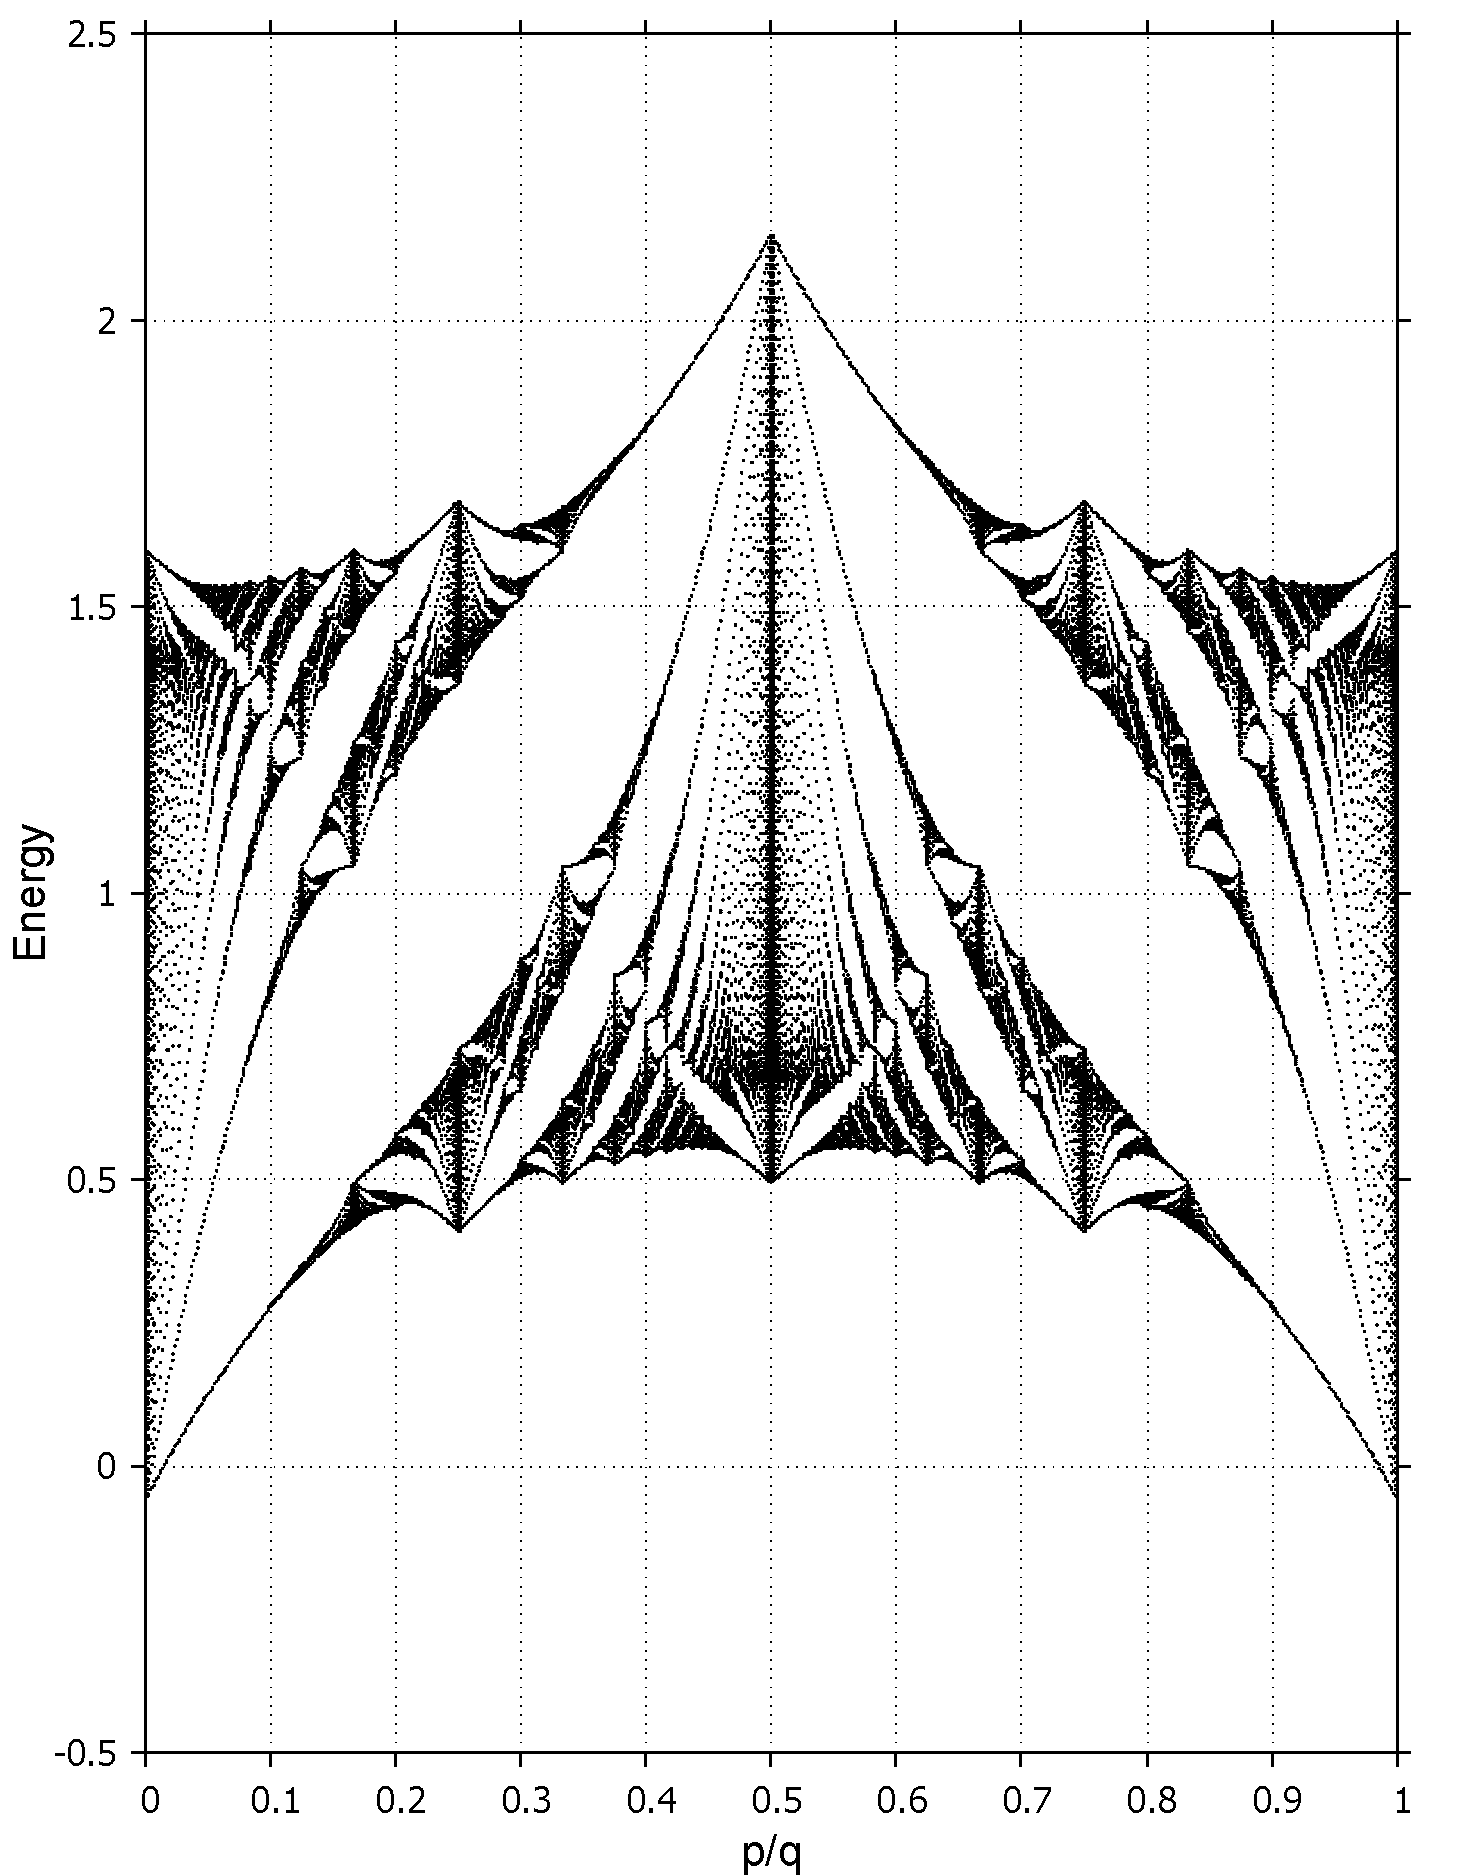
\includegraphics[width=0.85\textwidth,height=1.2\linewidth]{pic/h0_tam giac_q_797.png}
		\label{fig:3 band}
	\end{subfigure}
	\begin{subfigure}[b]{0.495\textwidth}
		\centering
		\includegraphics[width=0.85\textwidth,height=1.2\linewidth]{pic/3band_gnuplot_q_797.png}
		\label{fig:1 band}
	\end{subfigure}
	\caption{
		Hofstadter butterfly for one band $\ket{dz} \equiv \ket{\phi_{1}^{1}(x,y)}$(left) and all band(right) with $q = 797$ and vary $p$  from 1 to $q$ with field strength $B_{0} = 4.6928 \times 10^{4}$ T. Here on $x-$axis represents the flux in units of quantum flux enclosed by the unit cell and $y-$axis represents the Energy.
	}
\end{figure*}

The magnetic field enters the TB Hamiltonian only through the fraction $p/q$, which is the magnetic flux through the primitive unit cell of the lattice. In general, as the lattice geometry evolves, the area of the primitive unit cell changes $(m + 1/2)$ times. \\
Another observation is that the lattice constant $a$ and the magnetic field $B$ always appears together in an expression with the magnetic field ($\tfrac{Ba^{2}\sqrt{3}}{4}$). This quantity reflects the flux per plaquette in the super magnetic unit cell, which is relevant is the context of Aharonov-Bohm effect \cite{aharonov1959}. Since the expression involves the product $Ba^{2}$, this implies that increasing $B$ by a certain amount is mathematically equivalent to increasing $a$. In other words, for energy calculations, increasing the strength of the magnetic field is physically equivalent to increasing the lattice constant, as both affect the system in the same way through the flux per unit cell.

The spectrum has various symmetries: It is only show that the flux $q$ is affects the spectrum, so if $p/q$ changed to $p/q + c$ while $c$ any interger, the spectrum is unchanged. The spectrum is also unchanged on changing $p/q$ to $-p/q$, because if $\psi$ is an eigenstate withe energy for field $p/q$, then its complex conjugate $\psi^{*}$ is an engenstate with the same energy for field $-p/q$. These two symmetries are not special to the $MX_{2}$'s case. The third symmetry is that if $p/q$ is changed to $p/q + 1/2$, this is the same as changing $t_{i}$, which are hopping energies, to $-t_{i}$, this leads to the inverting of the spectrum.

Before we end the section, a few general remarks are in order. The role of the eight hopping constants $t$ is just to set an energy scale. Change the hopping constants amounts to stretching the butterfly spectrum vertically, which is an overall scaling to the energy levels. Thus it does not give rise to any interesting physical phenomenon.
\begin{figure*}[htb]
	\centering
	\begin{subfigure}[b]{0.32\linewidth}
		\centering
		\includegraphics[width=0.95\textwidth,height=1.2\linewidth]{pic/plotHofstadterButterfly_q=797_MoS2.png}
		\label{fig:matt 1}
	\end{subfigure}
	\begin{subfigure}[b]{0.32\linewidth}
		\centering
		\includegraphics[width=0.95\textwidth,height=1.2\linewidth]{pic/plotHofstadterButterfly_q=797_MoSe2.png}
		\label{fig:matt 2}
	\end{subfigure}
	\begin{subfigure}[b]{0.32\linewidth}
		\centering
		\includegraphics[width=0.95\textwidth,height=1.2\linewidth]{pic/plotHofstadterButterfly_q=797_MoTe2.png}
		\label{fig:matt 3}
	\end{subfigure}
	\begin{subfigure}[b]{0.32\linewidth}
		\centering
		\includegraphics[width=0.95\textwidth,height=1.2\linewidth]{pic/plotHofstadterButterfly_q=797_WS2.png}
		\label{fig:matt 4}
	\end{subfigure}
	\begin{subfigure}[b]{0.32\linewidth}
		\centering
		\includegraphics[width=0.95\textwidth,height=1.2\linewidth]{pic/plotHofstadterButterfly_q=797_WSe2.png}
		\label{fig:matt 5}
	\end{subfigure}
	\begin{subfigure}[b]{0.32\linewidth}
		\centering
		\includegraphics[width=0.95\textwidth,height=1.2\linewidth]{pic/plotHofstadterButterfly_q=797_WTe2.png}
		\label{fig:matt 6}
	\end{subfigure}
	\caption{
		The Hofstadter’s butterflies of $MX_{2}$ monolayers using GGA parameters from Table 1.
	}
\end{figure*}


%Using Eq (2.16), we obtain the eigenvalue equation $H \phi_{\mu}^{j} = E \phi_{\mu}^{j}$ and


% t_{0} e^{- i \left(2  \pi (m + \frac{1}{2}) \eta + k_{y} a \frac{\sqrt{3}}{2}\right) }
An alternative approach to the derivation of the Hamiltonian under an uniform magnetic field is given in \hyperref[appendix b]{Appendix B}.
%\newpage
%\section{Spin-orbit coupling}

Due to the heavy mass of the transistion-metal $M$ atom, its \ac{SOC} can be large. For the sake of simplicity, only the on-site contribution, namely, the $\mathbf{L \cdot S}$ term from $M$ atoms.\\ By using the bases $\left\{\ket{d_{z^{2}},\uparrow},\ket{d_{xy},\uparrow},\ket{d_{x^{2} - y^{2}},\uparrow},\ket{d_{z^{2}},\downarrow},\ket{d_{xy},\downarrow},\ket{d_{x^{2} - y^{2} },\downarrow}\right\}$, we get the SOC contribution to the Hamiltonian as
\begin{gather}
	H{'}
	= \lambda \mathbf{L \cdot S}
	= \f{\lambda}{2}
	\begin{pNiceMatrix}
		L_{z}           & L_{x} - i L_{y} \\
		L_{x} + i L_{y} & -L_{z}
	\end{pNiceMatrix},
\end{gather}
in which
\begin{gather}
	L_{z}
	=
	\begin{pNiceMatrix}
		0 & 0   & 0  \\
		0 & 0   & 2i \\
		0 & -2i & 0
	\end{pNiceMatrix},
\end{gather}
is the matrix of $\hat{L}_{z}$ ($z$ component of the orbital angular momentum) in bases of $d_{z^{2}},d_{xy},d_{x^{2} - y^{2}}$ and $\lambda$ is characterized the strength of the SOC. Noting that, under the three bases, the matrix elements of $\hat{L}_{x}$ and $\hat{L}_{y}$ are all zeros. Therefore the full TB Hamiltonian for the magnetic unit cell with the SOC as follows
\begin{equation}
	\begin{aligned}
		H_{\text{SOC}}(\mathbf{k})
		 & = \mathbf{I}_{2} \otimes H_{0}(\mathbf{k}) + H{'} \\
		 & =
		\begin{pmatrix}
			H_{3q \times 3q}(\mathbf{k}) + \frac{\lambda}{2} L_{z} & 0                                                      \\
			0                                                      & H_{3q \times 3q}(\mathbf{k}) - \frac{\lambda}{2} L_{z}
		\end{pmatrix},
	\end{aligned}
\end{equation}
in which $I_{2}$ is the $2\times 2$ identity matrix and $H_{0} = H^{\text{NN}}$. To obtain the band structure, the eigenvalue of the Hamiltonian needs to be found at each


\begin{figure*}[htb]
	\begin{subfigure}[b]{0.495\textwidth}
		\centering
		\includegraphics[width=0.85\textwidth,height=1.2\linewidth]{pic/bandstructureSOC.pdf}
		%\caption{\label{band structure SOC}}
	\end{subfigure}
	\begin{subfigure}[b]{0.495\textwidth}
		\centering
		\includegraphics[width=0.85\textwidth,height=1.2\linewidth]{pic/plotHofstadterButterfly_q=797_MoS2_SOC.png}
		%\caption{\label{HB SOC}}
	\end{subfigure}
	\caption{Band structure of monolayer $MoS_{2}$ along $\Gamma$-K direction, SOC causes huge spin splittings in band-structure at $K$ and $-K$ points.}
\end{figure*}




\newpage
\section{Landau levels}
In solid-state physics, the behavior of electrons in magnetic fields is usually introduced by using the Hamiltonian
\begin{gather}
	H = \f{\mathbf{p} + e \mathbf{A}(\mathbf{r})^{2}}{2m} ,
\end{gather}
and the energy eigenfunctions are known as \ac{LLs}
\begin{gather}
	E_{n} = \left(n + 1/2\right) \hbar \omega_{c}.
\end{gather}

This treatment is for free electrons, but near the bottom of the two-dimensional tight-binding band of TMD we must find a regime in which the electron behaves as a nearly one(At least with a nearly free dispersion relation). \\
Recalling the result obtained for the dispersion relation of an electron within the tight binding model
\begin{gather}
	h_{0} = 2 t_{0} (\cos 2\alpha + 2 \cos \alpha \cos \beta) + \epsilon_{1},
\end{gather}
The dispersion energy is approximately free-electron-like by Taylor expansion to second order of $\mathbf{k}$
\begin{equation}
	\begin{aligned}
		h_{0}(\mathbf{k})
		 & \approx 2 t_{0} \left[1 - \frac{a^{2} k_{x}^{2}}{2} + 2\left(1 - \f{a^{2} k_{x}^{2}}{8}\right)\left(1 - \f{3a^{2} k_{y}^{2}}{8}\right)\right] \\
		 & = t_{0} \f{3}{16} \left(32 + a^{4} k_{x}^{2} k_{y}^{2}\right) - t_{0} \f{3}{2} a^{2}\left(k_{x}^{2} + k_{y}^{2}\right) + \epsilon_{1} ,
	\end{aligned}
\end{equation}
the first term $a^{2}$ is negligibly small and another can be treated like constant, then we have
\begin{equation}
	\begin{aligned}
		h_{0}(\mathbf{k})
		 & \approx 6 t_{0} - \f{3}{2} t_{0} a^{2} (k_{x}^{2} + k_{y}^{2}) + \epsilon_{1}.
	\end{aligned}
\end{equation}
One of the ways derivation of effective mass $m^{*}$ is substitution $\hbar\mathbf{k} \rightarrow \mathbf{\Pi} + e \mathbf{A}$, with Landau gauge $\mathbf{A} = (0,Bx,0)$
\begin{equation}
	\begin{aligned}
		h_{0}(\mathbf{\Pi})
		 & \approx 6 t_{0} - \f{3}{2} t_{0} \f{a^{2}}{\hbar^{2}} \left[ \Pi_{x}^{2} + \left(\Pi_{y} + e B x\right)^{2}\right] + \epsilon_{1}                                                           \\
		 & \approx 6 t_{0} - \f{3}{2} t_{0} \f{a^{2}}{\hbar^{2}} \Pi_{x}^{2} - \f{3}{2} t_{0} \f{a^{2}}{\hbar^{2}} (e B)^{2} \left[ x - \left(- \f{\hbar k_{y}}{eB}\right) \right]^{2} + \epsilon_{1}.
	\end{aligned}
\end{equation}
The Eq (2.24) can be rewrite in the form as
\begin{gather}
	E(\mathbf{\Pi}) = 6 t_{0} - \left[\f{1}{2m^{*}} \Pi_{x}^{2} + \f{1}{2} m^{*} \omega_{c}^{2}(x - x_{0})^{2}\right] + \epsilon_{1},
\end{gather}
where $m^{*} = \frac{\hbar^{2}}{3t_{0}a^{2}}$ is the effective mass and $x_{0} = \frac{\hbar k_{y}}{eB}$. Hence, the cyclotron frequency is
\begin{gather}
	\omega_{c} = \f{eB}{m^{*}} = \f{8 \pi \sqrt{3} t_{0}}{\hbar}  \f{p}{q},
\end{gather}
and therefore the Landau levels near the bottom of the band structure can be written as
\begin{equation}
	\begin{aligned}
		E_{n}
		 & = 6 t_{0} - \hbar \omega_{c} (n + 1 /2) + \epsilon_{1}                    \\
		 & = t_{0} \left(6 - 8\pi\sqrt{3} \f{p}{q}( n + 1 /2)\right) + \epsilon_{1},
	\end{aligned}
\end{equation}
in linear order of an uniform-flux, where $n$ is Landau index. These levels give rise to what is called ``the Landau fan'', being very important in the de Haas-van Alphen and Shubnikov-de Haas effects \cite{10.1119/1.1615568} which predicts oscillations of the magnetic moment of a meltal depending on an applied magnetic field.
\begin{figure*}[htb]
	\centering
	\begin{subfigure}[b]{0.49\textwidth}
		\centering
		{\includegraphics[width=0.85\textwidth,height=1.2\linewidth]{pic/small_area_LL.png}}
	\end{subfigure}
	\begin{subfigure}[b]{0.49\textwidth}
		\centering
		\includegraphics[width=0.85\textwidth,height=1.2\linewidth]{pic/landaulevel_h0_q_797_EF_final.pdf}
	\end{subfigure}
	\caption{
		(a) Same plot as Fig 2.3 but considering a small area and (b) shows superposition of the Landau fan diagram and the Hofstadter butterfly. Display the first $n = 30$ levels near the bottom of the conduction band for a magnetic field up to $B = 500$ T. The purple line in Fig 2.9(b) is supposed to be Fermi level. The Fermi energy is fixed at $E = 1.046$ eV.
	}
\end{figure*}

In Fig 2.9 we compare the spectrum of a small section of triangular lattice with $p / q = 1 / 797$, which is equivalent to small magnetic field, the spectrum of MoS$_{2}$, with the energy of Landau levels given by Eq. (2.50) show standard equally spaced LLs \cite{Shoenberg_1984,singleton2001band,blundell2001magnetism,kittel1987quantum} near the bottom of the bands, as plotted in Fig 2.9(b). The fan of LLs can be clearly seen emergin from the partern in Fig 2.9(a).

In Fig 2.9(a), there is just single-band in case zero field, with the effective mass $m^{*} = \frac{\hbar}{3 t_{0} a^{2}}$. The numerical result for this portion of the spectrum are shown in Fig 2.9 for $p/q \geq 1/797$. The first few LLs are clearly seen, and the asymtotic slopes $p/q$ at large $q$ given by Eq. (2.50) are shown for comparison for the first five Landau levels at $B \leq 100$ T. At the values of $B$ the fit is not ideal, but it does seem to be improving with the decreasing $p/q$. In our model study, LLs can be classified into specific groups. In each group, each levels can be further labeled by a Landau index $n$.

Figure 2.9 displays a blowup of the low uniform magnetic region and the LLs as a function of $\Phi / \Phi_{0}$ \cite{Li_2011}. The Fermi energy is supposed to be for $E_{F} = 1.046$ eV, this is, is plotted for one-half spectrum. The Landau levels are all close to being linear in $B$, resulting from the magnetic quantization of parabolic bands at $B = 0$ T i.e. increasing values of B, these LLs are sequentially depleted; for $B=200$ T the levels are completely filled up to the level $n=10$; for $B = 500$ T it happens the same, only this time are filled up to the level $n=4$ and so on.

%More interesting is the top and bottom of conduction and valence band of the zero field spectrum. This results in a non-standard Landau levels when the field is turned on, as discused above.\\
%In the one-band case, knowing the effective mass in zero field and the charge is enough to determine the Landau level spectruc to linear order in the magnetic field. For the three-band case
%
%
% In order to determine the cyclotron frequency for the three-band, through the derivation in Appendix C, we have obtained the Landau levels for the three-band model when the field is turned on
%\begin{figure*}[htb]
%	\centering
%	\begin{subfigure}[b]{0.49\textwidth}
%		\centering
%		{\includegraphics[width=0.85\textwidth,height=1.2\linewidth]{pic/small_area_LL_3band.png}}
%	\end{subfigure}
%	\begin{subfigure}[b]{0.49\textwidth}
%		\centering
%		\includegraphics[width=0.85\textwidth,height=1.2\linewidth]{pic/landaulevel_3band_q_797_EF_final.pdf}
%	\end{subfigure}
%	\caption{
%		test
%	}
%\end{figure*}
%Ta có thể thấy một số mức Landau có năng lượng là được tăng tuyến tính theo cường độ từ trường, nhưng lại không cách đều và chính xác như hình của Hofstadter butterfly. Thêm vào đó có nhiều trạng thái mà năng lượng tại đó thì giảm trong khi đó thì từ trường lại tăng. những trạng thái này sẽ được gọi là những trạng thái ``kì cục'' mà ta sẽ bàn luận ở đây.\\
%Trong trường hợp một band, khối lượng hiệu dụng $m^{*}$ và điện tích là đủ để mô tả được phổ Landau theo sự thay đổi tuyến tính của từ trường. Trong trường hợp 2 band và 3 band thì


%It is this fan of Landau levels that responsible for the de Haas-van Alphen and Shubnikov-de Haas effects.

\section{Hall effects}
\subsection{Introduction}
In this section, we will discuss the \ac{IQHE} where the flux number and flux quanta is a integer number. This phenomenon can be understood without taking into account the interactions between electrons. This means that we continue using the single particle Hamiltonian that we described in Section 2.

\subsection{The classical Hall effect}
An electric field $\mathbf{E}$ established in the solid results in a current density $\mathbf{J}$ linearly related to the field through Ohm's law
\begin{gather}
	\mathbf{J} = \boldsymbol{\sigma} \mathbf{E},
\end{gather}
where $\boldsymbol{\sigma}$ is the conductivity tensor. The structure of the matrix, with identical diagonal components, and equal but opposite off-diagonal components, follows from rotational invariance.

The resistivity is defined as the inverse of the conductivity. This remains true when both are tensors
\begin{equation}
	\begin{aligned}
		\rho = \sigma^{-1} =
		\begin{pNiceMatrix}
			\rho_{xx}  & \rho_{xy} \\
			-\rho_{xy} & \rho_{yy}
		\end{pNiceMatrix}
	\end{aligned},
\end{equation}
The off-diagonal components of resistivity tensor is $\rho_{xy} = \rho_{xy} = \tfrac{B}{en}$. Usually we measure the resistance $R$, which differs from the resistivity $\rho$ by geometric factors. However, for $\rho_{xy}$, this thing coincide. To see this, consider a sample of material of length $L$ in the $y$-direction. We drop a voltage $V_{y}$ in the $y$-direction and measure the resulting current $I_{x}$ in the $x$-direction. The transverse resistance is
\begin{gather}
	R_{xy} = \frac{V_{y}}{I_{x}} = \frac{L E_{y}}{L J_{x}} = \frac{E_{y}}{J_{x}} = -\rho_{xy}.
\end{gather}
For a current $I_{x}$ flowing in the $x$-direction, and the corresponded electric field $E_{y}$ in the $y$-direction, the Hall coefficent is defined by
\begin{gather}
	R_{H} = \frac{\rho_{xy}}{B} = \frac{1}{en} .
\end{gather}
We see that the Hall coefficent depends only on microscopic information about the material: the charge and density of conduction particles. The Hall coefficent does not depend on the scattering time $\tau$; it remains unaffected by the specific frictional mechanism present in the material.
\begin{figure*}[htb]
	\centering
	\begin{subfigure}[b]{0.495\textwidth}
		\centering
		{\includegraphics[width=0.83\textwidth,height=0.8\textwidth]{pic/classRess.pdf}}
	\end{subfigure}
	\begin{subfigure}[b]{0.495\textwidth}
		\centering
		\includegraphics[width=0.83\textwidth,height=0.8\textwidth]{pic/HallRess.pdf}
	\end{subfigure}
	\caption{
		The longitudinal resistance on the right figure and the Hall resistance in the left figure. The graph shows both the longitudinal resistance and the Hall resistance is linear to the increasing magnetic field.
	}
\end{figure*}
\subsection{The Quantum Hall effect}
In two dimensional, there is a crucial relationship between the conductivity tensor $\boldsymbol{\sigma}$ and the resistivity tensor $\boldsymbol{\rho}$ is given by
\begin{equation}
	\begin{aligned}
		\begin{bmatrix}
			\sigma_{xx} & \sigma_{xy} \\
			\sigma_{yx} & \sigma_{yy}
		\end{bmatrix}
		\begin{bmatrix}
			\rho_{xx} & \rho_{xy} \\
			\rho_{yx} & \rho_{yy}
		\end{bmatrix}^{-1}
		=
		\f{1}{\rho_{xx} \rho_{yy} - \rho_{xy} \rho_{yx}}
		\begin{bmatrix}
			\rho_{yy}  & -\rho_{xy} \\
			-\rho_{yx} & \rho_{xx}
		\end{bmatrix}
	\end{aligned}.
\end{equation}
In the previous study, we had arrived at the classical Hall resistance. And this remains stable as expect whenever we still trust classical mechanics. But the world is also consist quantum mechanics. This becomes important at low temperatures and strong magnetic fields.

There are two related phenomena which are associated to two different quantum Hall effects. These are called the integer and fractional quantum Hall effects. In this work, we first discovered and subsequenly understood theoretically the integer quantum Hall effect in the Hofstadter butterfly.

Let's take a look at the experimental data for the quantum Hall effect were perfomed in 1980 by von Klitzing \textit{et at.} \cite{klitzing90}
\begin{figure}[H]
	\centering
	\includegraphics[width=0.85\textwidth,height=0.45\linewidth]{pic/quantumhall.jpg}
	\caption{This is the integer quantum Hall effect. For this von Klitzing was awarded the 1985 Nobel prize.}
\end{figure}
\noindent Both the Hall resistivity $\rho_{xy}$ and the longitudinal resistivity $\rho_{xx}$ depict interesting behaviour. Perhaps the most striking feature in the figure is the fact that the Hall resistivity $\rho_{xy}$ sits on a plateau for a range of magnetic field, before jumping dramaticly to the next plateau. On these plateau, the Hall resistance now defined
\begin{gather}
	\rho_{xy} = \frac{R_{K}}{\nu}, \quad \nu = 1,2,...
\end{gather}

The contribution to the Hall conductance from a single subband is given by \cite{kohmoto1989,hatsugai1990energy,kohmoto1985topological,thouless1982}
\begin{gather}
	\sigma_{xy} = \f{e^{2}}{h} \sum_{n}^{\text{occ.}} \f{1}{2\pi} \oiint_{\text{Bz}} d k_{x} d k_{y} \Omega_{n}^{z} (\mathbf{k}),
\end{gather}
In general, the Berry curvature intergrated over a closed manifold is quantized in the units of $e^{2} / h$ and equals to the net number of monopoles inside. This number is called the Chern number and is responsible for a number of quantization effects. Therefore the Hall conductivity is quantized for a two dimensional band insulator of noninteracting electrons.
\subsection{Colored the spectrum}
With the cyclotron frequency in Section 2.4, the electron energy is quantized to the Landau levels.

We calculate the quantum Hall conductivity by the Streda formula \cite{streda1982}
\begin{gather}
	\sigma_{xy}(B,E_{F}) = e \f{\partial \rho (E_{F},B)}{\partial B},
\end{gather}
where $\rho(E_{F},B)$ is the cumulative energy density of state at Fermi-energy $E_{F}$. As show in Fig, the Hall conductivity is quantized at colored points. Since the intergral for the whole Brillouin zone respectively Berry curvature, we arrived at the Thouless-Kohmoto-Nightingale-Nijs's formula (TKNN)
\begin{gather}
	\sigma_{xy} = \f{e^{2}}{h} \nu, \quad \nu = 1,2,..
\end{gather}
$\nu$ is guaranteed to be an integer given by the Chern number. Combining Eq(2.39) and Eq(2.40), we have
\begin{gather}
	\f{\partial \rho}{\partial B} = \f{e}{h} \nu.
\end{gather}

Assuming that $B$ has slight variation
\begin{gather}
	\rho = \text{const} + \f{e}{h}B \nu.
\end{gather}
Before this, we have defined $\frac{p}{q} = \frac{eBa^{2}\sqrt{3}}{4h}$, with $S = \frac{\sqrt{3} a^{2}}{4}$ is the area of the unit cell. Multiply $S$ with Eq(2.42), we have
\begin{gather}
	\rho \times S = \text{const} + \f{p}{q} \nu,
\end{gather}
and the density of electron in a single band is given by $\frac{1}{Sq}$, thus when there are $r$ band below the Fermi energy level, the density of electron for $r$-{\text{th}} bands is
\begin{gather}
	\rho = \f{r}{Sq}.
\end{gather}
The Eq(2.42), then, is written as,
\begin{gather}
	r = \text{const} \times q + p \times \nu_{r},
\end{gather}
in this equation $r,q,p,\nu_{r}$ are intergers, thus, const$\times q$ must be an interger. On the one hand, since const is independent of $q$, and $q$ can change when the magnetic field is varied without making a point of contact, then const itself must be an interger, namely $s_{r}$. Thus we have
\begin{gather}
	r = q \times s_{r} + p \times \nu_{r},
\end{gather}
which is the Diophantine equation. In order to compute the Hall conductivity of the lattice model for a electron in a background magnetic field. We can only do this for rational fluxes $\frac{\Phi}{\Phi_{0}} = \frac{p}{q}$. In this case, we can use the TKNN formula, but with the Chern number, which used to be defined by intergrating over the Brillouin zone, now arising by intergrating over the magnetic Brillouin zone. Others derivation is in \cite{di2022linking},\cite{dana1985}.

The Hofstadter butterfly may be colored in a various ways. For instance, we may color the points of the butterfly by their Chern number, as illustrated in the Fig2.11(a). The disadvantage of this, is that there will be many points in the butterfly and so the fine details of the coloring may be obscured.
\begin{figure*}[htb]
	\centering
	\begin{subfigure}[b]{0.495\textwidth}
		\centering
		{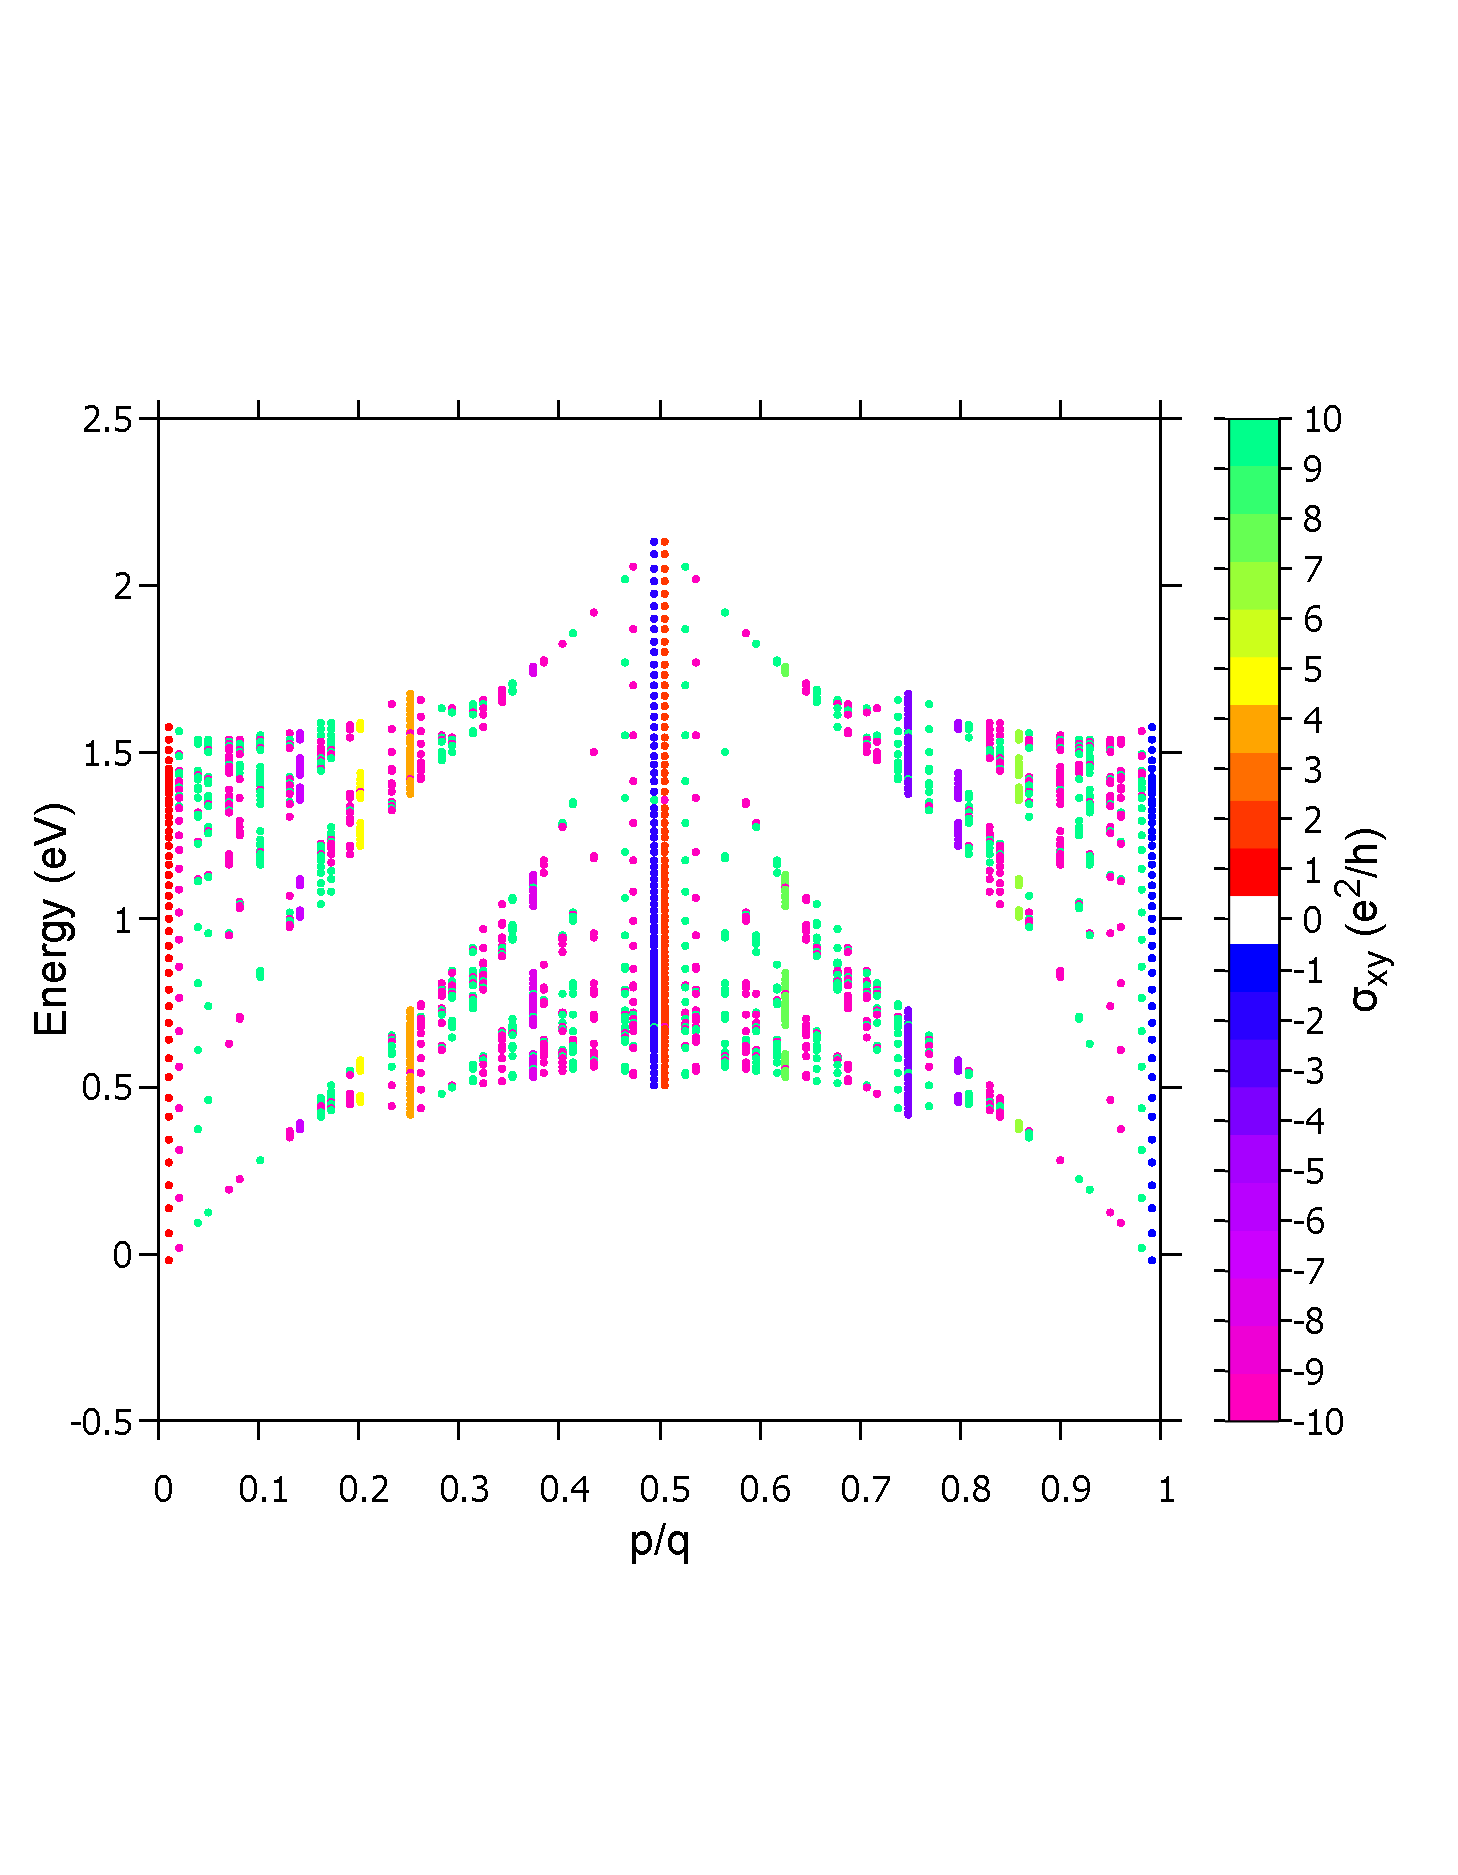
\includegraphics[width=0.85\textwidth,height=1.2\linewidth]{pic/1band_Chern_q_99.png}}
	\end{subfigure}
	\begin{subfigure}[b]{0.495\textwidth}
		\centering
		\includegraphics[width=0.85\textwidth,height=1.2\linewidth]{pic/1band_Chern_q_797_colorplane.png}
	\end{subfigure}
	\caption{
		q = 99 và q = 797
	}
\end{figure*}
%	\begin{subfigure}[b]{0.495\textwidth}
%	\centering
%	\includegraphics[width=0.85\textwidth,height=1.2\linewidth]{pic/wannier_gnu.pdf}
%\end{subfigure}

Fig 2.11(b) shows the Hofstadter butterfly, color-coded according to the Hall conductance. Moreover, the Chern number magnitude range will increase with $q$ and so it is difficult to define a fixed scale. In this work, we uses a scale for Chern numbers with magnitude up to 10, as well as the color palette made famous by Avron $et \; al.$ \cite{avron2003}. Any Chern number out of range $-10 \leq \nu \leq 10$ is equal to zero. Regions with zero Hall conductance and the corresponding spectrum are left blank. The two largest gaps near the center of the figure are associated with small intergers where the color coding is faithful. The colored picture emphasizes the gaps while the standard Hofstadter butterfly emphasis the spectrum. The colored figure is prettier and displays the regular aspects of the diagram: gaps exhibit better-defined behavior than spectra.

The transverse conductane in each energy gap, depicted in figure, is given by the sum of the Chern numbers of the occupied bands. At first discussed by Wannier in refernce \cite{wannier1978}, even a small change in the flux modifies radically the underlying band structure, thereby altering the intergrated density of states.

This results consistent with the Quantumm Hall effect and the Shubnikov-de Haas effects.



\subsection{Solving the diophantine equation}
We have defined that the magnetic flux through a unit cell is $\frac{\Phi}{\Phi_{0}} = \frac{p}{q}$. For $p$ and $q$ are mutually prime numbers, we defined the pairs $(\nu_{r},s_{r})=(m,n)$ as the solutions
\begin{gather}
	p m + q n  = \gcd(p,q).
\end{gather}
Fortunately, $p$ and $q$ are co-prime, Eq (2.47) is now
\begin{gather}
	pm + qn = 1,
\end{gather}
By deviding $p$ by $q$, we get a quotient $a$ and a remainder $b$. They satisfy
\begin{gather}
	q = p a + b.
\end{gather}
By using the Euclidean Algorithm, we can easily find $(m,n)$. For instance, the rational magnetic flux is $\frac{p}{q} = \frac{30}{47}$, then the diophantine equation now is $30m + 47n = 1$, and
\begin{equation}
	\begin{aligned}
		47 = 30 \times 1 + 17, \\
		30 = 17 \times 1 + 13, \\
		17 = 13 \times 1 + 4,  \\
		13 = 4 \times 3 + 1.   \\
	\end{aligned}
\end{equation}
At this point we stop, because we arrived at the greatest common divisor, so the algorithm is over. The next step is solve for the remainders
\begin{equation}
	\begin{aligned}
		47 = 30 \times 1 + 17 \Rightarrow 17 = 47 \times 1 + 30 \times (-1), \\
		30 = 17 \times 1 + 13 \Rightarrow 13 = 30 \times 1 + 17 \times (-1), \\
		17 = 13 \times 1 + 4 \Rightarrow 4 = 17 \times 1 + 13 \times (-1),   \\
		13 = 4 \times 3 + 1 \Rightarrow 1 = 13 \times 1 + 4 \times (-3).
	\end{aligned}
\end{equation}
We are going to take this last remainder equation, and do backwards substitute until we get the very first remainder
\begin{equation}
	\begin{aligned}
		1 & = 13 \times 1 + 4 \times (-3)                              \\
		  & = 13 \times 1 + [17 \times 1 + 13 \times (-1)] \times (-3) \\
		  & = 13 \times 4 +17 \times (-3)                              \\
		  & = [30 \times 1 + 17 \times (-1)] \times 4 + 17 \times (-3) \\
		  & = 30 \times 4 + 17 \times (-7)                             \\
		  & = 30 \times 4 + [47 \times 1 + 30 \times (-1)] \times (-7) \\
		  & = 30 \times (11) + 47 \times (-7),
	\end{aligned}
\end{equation}
we find the solution for $(m,n)$ is $(11,-7)$.
\subsection{Wannier diagram}
To further explore the intricate fractal nature of the Hofstadter spectrum, we shall now achieve a simplified replica of Fig, a powerful tool for visualizing the relationship between magnetic flux and electron filling in the system. Wannier's diagram provides a graphical representation of the allowed energy gaps in the Hofstadter spectruc as a function of the magnetic flux per unit cell and the electron filling factor. This diagram is particularly insightful because it captures the topological properties of the system through the distribution and behavior of these energy gaps.

The fundamental of Wannier's diagram lies in the Diophantine gap equation
\begin{gather}
	\f{n}{n_{0}} = \nu \f{\Phi}{\Phi_{0}} + s,
\end{gather}
where $\frac{n}{n_{0}}$ is the electron filling factor, representing the ratio of the number of electrons per unit cell, $\nu$ is the Chern number associated with the quantized Hall conductance, and $s$ is another interg that corresponds to the gap index, effectively indicationg the electron filling within the spectrum.

The Diophantine equation is crucial in understanding the quantization of Hall conductance in the Hofstadter butterfly. The Chern number $t$ dertermines the topological nature of the bands and their contribution to the Hall conductance, while the interger $s$ identifies specific energy gaps in the spectrum. These gaps are directly linked to incompressible quantum Hall states, which are of significant interest in both theoretical and experimental condensed matter physics.

The calculated Wannier's diagram, the energy density of state as a function of filling factor $\frac{n}{n_{0}}$ and magnetic flux $\Phi$ as illustrated in Fig, reveal the presence of these energy gaps across the spectrum. Each colored line in the diagram corresponds to an energy gap where the system exhibits an imcompressible quantumm Hall state, characterized by a quantized Hall conductance. The diagram not only provides a clear visuallization of the gap structure but also offers insights into the topological phases that arise in monolayer TMD systems under varying magnetic flux conditions.
\begin{figure}[H]
	\centering
	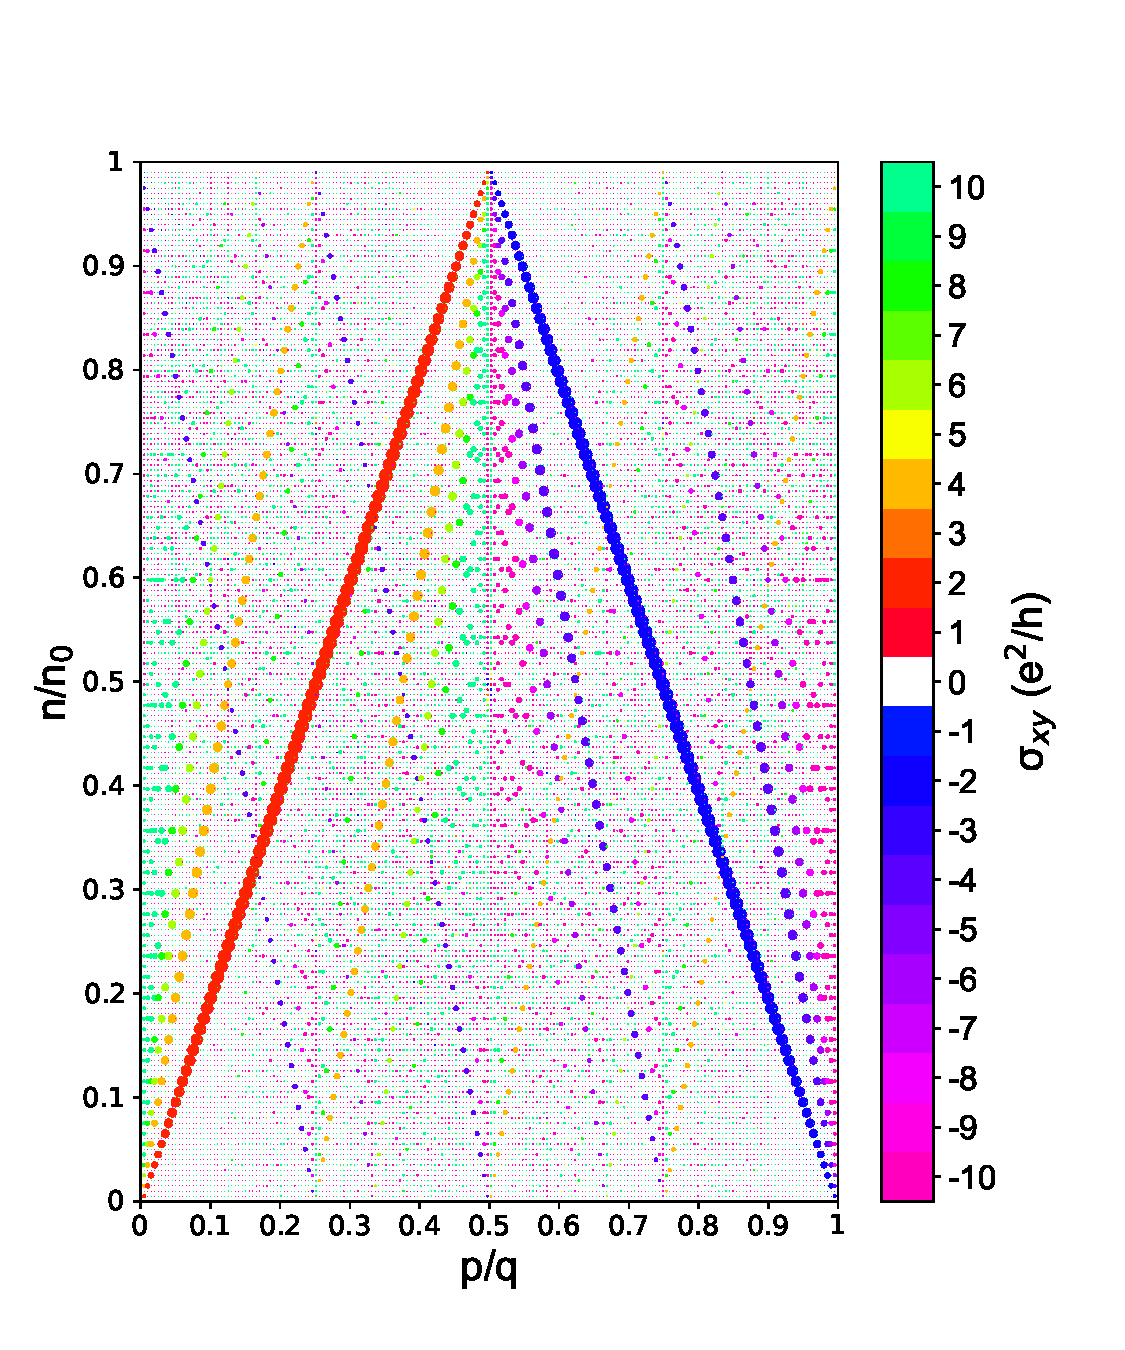
\includegraphics[width=0.8\textwidth,height=0.85\linewidth]{pic/wannier199.png}
	\caption{Wannier diagram}
\end{figure}

\chapter{RESULT AND DISCUSSION}
\chapter{CONCLUSION AND FUTURE WORK}
\section{Conclusion}
In our research, we have calculated the Hofstadter butterfly of monolayer MoS$_{2}$ and others transistion metal dichalcogenide types by using a tight-binding three-band model. In addition, we have explored the rich and complex physics of monolayer MoS$_2$, such as Landau levels and integer quantum Hall effect (IQHE), in the presence of external magnetic fields. The research conducted within these pages has demonstated the unique interplay between the superlattice and magnetic fields, which leads to the emergence of fascinating quantum phenomena. 

In section 2.1, we have studied the tight-binding three-band model for monolayers of MX$_{2}$ using only the M$-d_{z^{2}}$, $d_{xy}$ and $d_{x^{2} - y{^2}}$ orbitals. When only NN M-M hoppings are included, we calculated the hopping energies using the symmetry of the $D_{3h}$ point group we derived eights hopping parameters from Ref \cite{PhysRevB.88.085433}.

In section 2.2, we focused on the Hofstadter physics in monolayer TMD, where the lattice gives rise to a rich Hofstadter spectrum when subjected to a magnetic field. The detailed analysis revealed key features of the spectrum, including the SOC and the emergence of topological quantum Hall states. In addition, the study also demonstrated that there are many ways to derivive the Hofstadter spectrum two of those is using the Peierls substitution or Envelope Function Approximation.

In section 2.3 and section 2.4, extended the investigation into the realm of Hall effects, introducing the Landau levels, the interger quantum Hall effect and applying it to monolayer TMD systems. We also shown that how the Hofstadter butterfly can be colored in various ways using the Chern number.

Overall, while this study provides valuable insights, we acknowledge several limitations. Firstly, in section 2.3 and 2.4, our calculation was restrited to the single-band approximation due to the computational complexity of multi-band interactions. Specifically, incorporating three-band model would require significantly more resources, particularly in calculating Chern numbers, which are numerically intensive for larger Hamiltonian matrices. Secondly, for tractability, we adopted the convection from  Ref \cite{klitzing90} of fixing the Fermi energy at mid-spectrum. While this simplification is justified in certain regimes, it may not hold under strong magnetic field, where the density of electrons may be changed correspoding the magnetic field.
\section{Future work}
For further research, we can utilize thi




\appendix
\renewcommand{\chaptername}{Appendix}
%\chaptermark{Appendix}
%\begin{appendices}
%	\section{1}
%\end{appendices}

\chapter{Harper's equation} \label{appendix b}
%We now consider the Harper equation fo the case where the crystal lattice is a square lattice, given by the Hamiltonian from the example in the text \cite{yalcin_2019}
%\begin{equation}
%	\begin{aligned}
%		H(\mathbf{k})
%		 & = 2 t \left[\cos(k_{x} a) + \cos(k_{y} a)\right]                               \\
%		 & = t \left[ e^{ik_{x} a} + e^{-ik_{x} a} + e^{ik_{y} a} + e^{-ik_{y} a} \right]
%	\end{aligned}
%\end{equation}
%By using Peierls's substitution $\hbar\mathbf{k} \rightarrow (\mathbf{\Pi} - e \mathbf{A})$, ta có
%\begin{equation}
%	\begin{aligned}
%		H & = t \left[ e^{ik_{x} a} + e^{-ik_{x} a} + e^{i (p_{y} - e Bx) a/\hbar} + e^{-i (p_{y} - e Bx) a/\hbar} \right]                                    \\
%		  & = t \left[ e^{ik_{x} a} + e^{-ik_{x} a} + e^{i p_{y} a/\hbar} e^{i 2 \pi Bx / \Phi_{0}} + e^{-i p_{y} a/\hbar} e^{-i 2 \pi Bx / \Phi_{0}} \right]
%	\end{aligned}
%\end{equation}
%Substituting $x = ma$ and $y = na$ given the coordinates of the square lattice, we obtain the Harper equation
%
We now consider the case of hexagonal lattice with one band as a basis under an uniform magneticc field given by the Landau gauge $\mathbf{A} = (0, Bx,0)$. Given

\begin{equation}
	\begin{aligned}
		h_0
		 & = 2 t_0 \left(\cos2\alpha + 2\cos\alpha \cos\beta\right) + \epsilon_1                                                                                                                                     \\
		 & = 2t_{0} \left[ \cos(k_x a) + 2 \cos \left(\f{k_x a}{2}\right) \cos \left(\f{\sqrt{3}k_y a}{2}\right) \right] + \epsilon_1                                                                                \\
		 & = 2t_{0} \left\{ \cos(k_x a) + \cos\left[\left( k_{x} + \sqrt{3} k_{y} \right)\frac{a}{2}\right] + \cos\left[\left( k_{x} - \sqrt{3} k_{y} \right)\frac{a}{2}\right]\right\} + \epsilon_1                 \\
		 & = 2t_{0} \Biggl\{ \cos(\Pi_{x}\f{a}{\hbar}) + \cos \left[\left(\Pi_{x} + \sqrt{3} e B x + \sqrt{3} \Pi_{y}\right)\frac{a}{2\hbar}\right]                                                                  \\
		 & + \cos \left[\left(\Pi_{x} - \sqrt{3} e B x - \sqrt{3} \Pi_{y}\right)\frac{a}{2\hbar}\right] \Biggr\} + \epsilon_1                                                                                        \\
		 & = t_{0} \biggl[e^{i \Pi_{x}\frac{a}{\hbar}} + e^{-i\Pi_{x}\frac{a}{\hbar}} + e^{i(\Pi_{x} + \sqrt{3} eBx + \sqrt{3} \Pi_{y} ) a / 2\hbar} + e^{-i(\Pi_{x} + \sqrt{3} eBx + \sqrt{3} \Pi_{y} ) a / 2\hbar} \\
		 & + e^{i(\Pi_{x} - \sqrt{3} eBx - \sqrt{3} \Pi_{y} ) a / 2\hbar} + e^{-i(\Pi_{x} - \sqrt{3} eBx - \sqrt{3} \Pi_{y} ) a / 2\hbar} \biggr] + \epsilon_1.
	\end{aligned}
\end{equation}
We replaced $\hbar \mathbf{k}$ in the above function by the operators $\mathbf{\Pi} + e \mathbf{A} / c$ in order to create an operator out of $h_{0}$. This method can be related to Envelop Function Approximation(EFA). When this substitution is made, the Hamiltonian element is seen to contain translation operators $\exp[a \Pi_{x} / \hbar],\exp[a \sqrt{3} \Pi_{y} / (2\hbar)]$. Depending on the gauge chosen, there are, in addition, certain phase factors dependent on the magnetic field strength, which multiply the translation operators. The Landau gauge $\mathbf{A} = (0,Bx,0)$ was chosen, then only the translation along $y$ are multiplied by phases. \cite{PhysRevB.14.2239}However, we must be very careful regarding how the operators act on the wave functions, since $\left[x,\Pi_{x}\right] \neq 0$. In their article, Gumbs and Fekete \cite{gumps1997}  incorrectly applied the modified translation operators, leading to completely incorrect results. In this work, we treat the operators more correctly by applying the Baker-Campbell-Hausdorff(BCH) formula and taking into account the commutation relation $\left[x,\Pi_{x}\right] = i \hbar$
\begin{equation}
	\begin{aligned}
		e^{\pm i(\Pi_{x} + \sqrt{3} e B x) a / 2\hbar}
		 & = e^{\pm i \Pi_{x} a / 2 \hbar} e^{\pm i\sqrt{3} e B x a / 2 \hbar} e^{-\frac{1}{2} \left[\pm i \Pi_{x}, \pm i \sqrt{3} e B x\right] a^{2} / 2 \hbar^{2}} \\
		 & = e^{\pm i \Pi_{x} a / 2 \hbar} e^{\pm i\sqrt{3} e B x a / 2 \hbar} e^{\mp i \sqrt{3} e B a^{2} / 8 \hbar}.
	\end{aligned}
\end{equation}
Substituting $x = \f{ma}{2}$ into (B.2), this leads to
\begin{gather}
	e^{\pm i(\Pi_{x} + \sqrt{3} e B x) a / 2\hbar}
	= e^{\pm i \Pi_{x} a / 2 \hbar} e^{\pm i\sqrt{3} e B (m + 1 /2) a^{2} / 4 \hbar}.
\end{gather}
And
\begin{equation}
	\begin{aligned}
		e^{\pm i(\Pi_{x} - \sqrt{3} e B x) a / 2\hbar}
		 & = e^{\pm i \Pi_{x} a / 2 \hbar} e^{\mp i\sqrt{3} e B x a / 2 \hbar} e^{-\frac{1}{2} \left[\pm i \Pi_{x}, \mp i \sqrt{3} e B x\right] a^{2} / 2 \hbar^{2}} \\
		 & = e^{\pm i \Pi_{x} a / 2 \hbar} e^{\mp i\sqrt{3} e B x a / 2 \hbar} e^{\mp i \sqrt{3} e B a^{2} / 8 \hbar},
	\end{aligned}
\end{equation}
substituting $x = \f{ma}{2}$ into (B.4), this leads to
\begin{gather}
	e^{\pm i(\Pi_{x} - \sqrt{3} e B x) a / 2\hbar}
	= e^{\pm i \Pi_{x} a / 2 \hbar} e^{\mp i\sqrt{3} e B (m - 1 /2) a^{2} / 4 \hbar}.
\end{gather}
The operators $e^{\pm i \Pi_{x} a / 2 \hbar}, e^{\pm i \Pi_{y} \sqrt{3}a / 2 \hbar}$ can be regconized as translational operators, we can rewrite (B.3) as
%The time-indepentdent Schr\"{o}dinger's equation now becomes
\begin{equation}
	\begin{aligned}
		  & t_{0} \varphi_{0} (x + a,y) + t_{0}\varphi_{0} (x - a,y) + t_{0}\varphi_{0} (x + \frac{a}{2},y + \frac{a\sqrt{3}}{2}) e^{\frac{ie}{\hbar}B(m + 1 /2) \frac{a^{2}\sqrt{3}}{4}}                                                            \\
		+ & t_{0} \varphi_{0} (x + \frac{a}{2},y - \frac{a\sqrt{3}}{2}) e^{-\frac{ie}{\hbar}B(m + 1/2) \frac{a^{2}\sqrt{3}}{4}} + t_{0} \varphi_{0} (x - \frac{a}{2},y + \frac{a\sqrt{3}}{2}) e^{\frac{ie}{\hbar}B(m + 1/2) \frac{a^{2}\sqrt{3}}{4}} \\
		+ & t_{0} \varphi_{0} (x - \frac{a}{2},y - \frac{a\sqrt{3}}{2}) e^{-\frac{ie}{\hbar}B(m - 1/2) \frac{a^{2}\sqrt{3}}{4}} + \epsilon_{1} \varphi_{0}(x,y) = E_{1} \varphi_{0}(x,y),
	\end{aligned}
\end{equation}
for the sake of simplicity we have defined $\varphi_{0} \equiv \ket{d_{z^{2}}}$.\\
%We have established in Section 2.2 that when translated by a lattice vector $\mathbf{R}$, the wavefuntion for an electron in a periodic lattice picks up a phase correspondingly. This lets us define
%\begin{gather}
%	\varphi(x \pm a,y) = e^{\pm i k_{x} a} \varphi(x,y), \\ 
%	\varphi(x \pm \f{a}{2},y \pm \f{a\sqrt{3}}{2}) = e^{\pm i k_{x} \frac{a}{2}} e^{\pm i k_{y} \frac{a\sqrt{3}}{2}} \varphi(x,y).
%\end{gather}
%Substituting $x = m \f{a}{2}$ and $y = n \f{a\sqrt{3}}{2}$ for the given hexagonal lattice, we can express the time-indepentdent Schr\"{o}dinger equation as 
%\begin{equation}
%	\begin{aligned}
%		&t_{0} \varphi_{0}(m + 2, n) + t_{0} \varphi_{0}(m - 2, n) + t_{0} \varphi_{0}(m + 1, n + 1) e^{\frac{ie}{\hbar}Bm \frac{a^{2}\sqrt{3}}{4}} \\
%		+& t_{0} \varphi_{0}(m + 1, n - 1) e^{-\frac{ie}{\hbar}Bm \frac{a^{2}\sqrt{3}}{4}} + t_{0} \varphi_{0}(m - 1, n + 1) e^{\frac{ie}{\hbar}Bm \frac{a^{2}\sqrt{3}}{4}} \\
%		+& t_{0} \varphi_{0}(m - 1, n - 1) e^{-\frac{ie}{\hbar}Bm \frac{a^{2}\sqrt{3}}{4}} + \epsilon_{1} \varphi_{0}(m,n) = E_{1} \varphi_{0}(m,n).
%	\end{aligned}
%\end{equation}
It is reasonable to assume planewave behavior in the $y$ direction, since the coefficents in the above equation only involve $x$. Therefore, we can assume the partial solution for $y$ to be in the form
\begin{gather}
	\varphi(\frac{ma}{2},\frac{na\sqrt{3}}{2}) = e^{i k_{y} n \frac{a\sqrt{3}}{2}} \varphi(m),
\end{gather}
which reduces (B.6) to
\begin{equation}
	\begin{aligned}
		  & t_{0} \varphi_{0}(m + 2) + t_{0} \varphi_{0}(m - 2) + t_{0} \varphi_{0}(m + 1) e^{2 i \pi (m + 1 /2) p/ q} e^{i k_{y} a\sqrt{3} / 2}                              \\
		+ & t_{0} \varphi_{0}(m + 1) e^{-2 i \pi (m + 1 /2) p/ q} e^{-i k_{y} a\sqrt{3} / 2} + t_{0} \varphi_{0}(m - 1) e^{2 i \pi (m - 1 /2) p/ q} e^{i k_{y} a\sqrt{3} / 2} \\
		+ & t_{0} \varphi_{0}(m - 1) e^{-2 i \pi (m - 1 /2) p/ q} e^{-i k_{y} a\sqrt{3} / 2} + \epsilon_{1} \varphi_{0}(m) = E_{1} \varphi_{0}(m),
	\end{aligned}
\end{equation}
this is equivalent to Eq. 2.16 we have mentioned in Section 2.2. Equation B.8 is sometimes called ``Harper's equation''. \cite{harper1955general} Since different $m$ values give different equations, one reaches a unique set of equations when $\Phi / \Phi_{0}$ is a rational number $p / q$ and $m$ goes through $q$ different values, essentially resulting in the Hamiltonian matrix written for a magnetic unit cell enlarged in $x$ direction $q$ times.\\
In the case of TMD presented in \cite{PhysRevB.88.085433}, the contribution of the
$X$ atom has been neglected, leading to the transformation of the hexagonal crystal structure of TMD into a regular triangular lattice. From there, we can map the triangular lattice to the case of the square lattice. In the triangular lattice, it has been established that the translation operators must satisfy the Baker-Campbell-Hausdorff formula.

\chapter{Cyclotron frequency for all band}
%Given Hamiltonian
%\begin{equation}
%	\begin{aligned}
%		\tilde{H}^{NN}(\mathbf{k})
%		 & = W H^{NN}(\mathbf{k}) W^{\dagger} \\
%		 & =
%		\begin{pNiceMatrix}
%			\frac{1}{2}(h_{11} + h_{22} + 2 \Im[h_{12}])  & \frac{1}{\sqrt{2}}(h_{1}^{*} + i h_{2}^{*}) & \frac{1}{2} (h_{11} - h_{22} + 2 i \Re[h_{12}]) \\
%			\frac{1}{\sqrt{2}}(h_{1} - i h_{2})           & h_{0}                                       & \frac{1}{\sqrt{2}}(h_{1} + i h_{2})             \\
%			\frac{1}{2}(h_{11} - h_{22} - 2i \Re[h_{12}]) & \frac{1}{\sqrt{2}}(h_{1}^{*} - i h_{2}^{*}) & \frac{1}{2}(h_{11} + h_{22} - 2i \Im[h_{12}])
%		\end{pNiceMatrix}
%	\end{aligned}
%\end{equation}
%Hamiltonian matrix element for the valence band now is
%\begin{equation}
%	\begin{aligned}
%		h_{v}
%		= & \f{1}{2} \left(h_{11} + h_{22} + 2 \Im[h_{12}]\right)                                                                            \\
%		= & \left(t_{11} + t_{22}\right) \cos 2\alpha + 2 \left(t_{11} + t_{22}\right) \cos \alpha \cos \beta                                \\
%		  & + 4 t_{12} \sin \alpha (\cos \alpha - \cos \beta) + \epsilon_{2}                                                                 \\
%		= & \left(t_{11} + t_{22}\right) \cos k_{x} a + 2 \left(t_{11} + t_{22}\right) \cos \frac{k_{x}a}{2} \cos \frac{\sqrt{3} k_{y} a}{2} \\
%		  & + 4 t_{12} \sin \frac{k_{x}a}{2} (\cos \frac{k_{x}a}{2} - \cos \frac{\sqrt{3} k_{y} a}{2}) + \epsilon_{2}.
%	\end{aligned}
%\end{equation}
%By using Taylor's expansion to second order of $\mathbf{k}$ on (C.2) we have
%\begin{equation}
%	\begin{aligned}
%		h_{v}
%		\approx & (t_{11} + t_{22}) \left(1 - \f{a^{2} k_{x}^{2}}{2}\right) + 2 (t_{11} + t_{22}) \left(1 - \f{a^{2} k_{x}^{2}}{8}\right) \left(1-\f{3a^{2} k_{y}^{2}}{8}\right) \\
%		        & - 4 t_{12} \f{a k_{x}}{2} \left( \f{a^{2} k_{x}^{2}}{8} - \f{3a^{2} k_{y}^{2}}{8}  \right) + \epsilon_{2}                                                      \\
%		\approx & 3(t_{11} + t_{22}) - \f{3a^{2}(t_{11} + t_{22})}{4} \left(k_{x}^{2} + k_{y}^{2}\right) - \f{a^{3} t_{12} k_{x}\left(k_{x}^{2} - 3 k_{y}^{2}\right)}{4}         \\
%		        & + \f{6a^{4}(t_{11} + t_{22})}{32} k_{x}^{2} k_{y}^{2} + \epsilon_{2} .
%	\end{aligned}
%\end{equation}
Starting with using Taylor expansion to second order of $\mathbf{k}$ for Hamiltonian elements in Eq()
\begin{equation}
	\begin{aligned}
		h_{0}  & = t_{0} (6 - \frac{3}{2} a^{2} (k_{x}^{2} + k_{y}^{2})) + \epsilon_{1} ,                                                                         \\
		h_{1}  & = i t_{1} 3a k_{x} - \frac{3}{2} t_{2} a^{2} k_{x}k_{y}    ,                                                                                     \\
		h_{2}  & = 2 t_{2} (\frac{3}{8} a^{2} k_{x}^{2} + \frac{3}{8} a^{2} k_{y}^{2}) + i 3 t_{1} a k_{y}          ,                                             \\
		h_{11} & = (t_{11} + 3 t_{22}) (1 - \frac{1}{8}a^{2} k_{x}^{2} - \frac{3}{8}a^{2} k_{y}^{2}) + 2 t_{11}(1 - \frac{1}{2} a^{2} k_{x}^{2}) + \epsilon_{2} , \\
		h_{22} & = (3 t_{11} + t_{22}) (1 - \frac{1}{8}a^{2} k_{x}^{2} - \frac{3}{8}a^{2} k_{y}^{2}) + 2 t_{22}(1 - \frac{1}{2} a^{2} k_{x}^{2}) + \epsilon_{2} , \\
		h_{12} & = \sqrt{3} (t_{22} - t_{11}) a^{2} k_{x} k_{y}.
	\end{aligned}
\end{equation}
In this (C.1), we have neglected coefficents of terms $a^{3},a^{4}$ by the small of large limit $a$ this leads to
% this leads to
%\begin{gather}
%	h_{v} \approx 3(t_{11} + t_{22}) - \f{3a^{2}(t_{11} + t_{22})}{4} \left(k_{x}^{2} + k_{y}^{2}\right) - \f{a^{3} t_{12} k_{x} \left(k_{x}^{2} - 3 k_{y}^{2}\right)}{4} + \epsilon_{2},
%\end{gather}
and using substitution $\hbar\mathbf{k} \rightarrow (\mathbf{\Pi} + e\mathbf{A})$
\begin{equation}
	\begin{aligned}
		h_{0}  & = t_{0} (6 - \frac{3}{2\hbar^{2}} a^{2} (\Pi_{x}^{2} + (\Pi_{y} + e Bx)^{2})) + \epsilon_{1}  ,                                                                                          \\
		h_{1}  & = i t_{1} \frac{3}{\hbar}a \Pi_{x} - \frac{3}{2\hbar^{2}} t_{2} a^{2} \Pi_{x}(\Pi_{y} + eBx)       ,                                                                                     \\
		h_{2}  & = 2 t_{2} (\frac{3}{8\hbar^{2}} a^{2} \Pi_{x}^{2} + \frac{3}{8\hbar^{2}} a^{2} (\Pi_{y} + eBx)^{2}) + i \frac{3}{\hbar} t_{1} a (\Pi_{y} + eBx)     ,                                    \\
		h_{11} & = (t_{11} + 3 t_{22}) (1 - \frac{1}{8\hbar^{2}}a^{2} \Pi_{x}^{2} - \frac{3}{8\hbar^{2}}a^{2} (\Pi_{y} + eBx)^{2}) + 2 t_{11}(1 - \frac{1}{2\hbar^{2}} a^{2} \Pi_{x}^{2}) + \epsilon_{2}, \\
		h_{22} & = (3 t_{11} + t_{22}) (1 - \frac{1}{8\hbar^{2}}a^{2} \Pi_{x}^{2} - \frac{3}{8\hbar^{2}}a^{2} (\Pi_{y} + eBx)^{2}) + 2 t_{22}(1 - \frac{1}{2\hbar^{2}} a^{2} \Pi_{x}^{2}) + \epsilon_{2}, \\
		h_{12} & = \frac{\sqrt{3} (t_{22} - t_{11}) a^{2}}{\hbar^{2}} \Pi_{x} (\Pi_{y} + eBx).
		%+ 4i t_{12} \frac{a k_{x}}{2} ( \frac{3a^{2} k_{y}^{2}}{8} - \frac{a^{2} k_{x}^{2}}{8})
	\end{aligned}
\end{equation}
%Eq (C.5) can be written in th the form as
%\begin{gather}
%	h_{v} = 3 (t_{11} + t_{22}) - \left[\f{\Pi_{x}^{2}}{2m^{*}} + \f{1}{2}m^{*} \omega_{c}^{2}(x - x_{0})^{2}\right] + \epsilon_{2}
%\end{gather}
%where $m^{*} = \f{2\hbar^{2}}{3a^{2}(t_{11} + t_{22})}$ is the effective mass  and $x_{0} = -\frac{\hbar k_{y}}{eB}$ for near the top of the valence band.

Instead of doing as we have done in Section 2, there is an alternative way to determine the energy spectrum. The Hamiltonian can be simplified by a suitably chosen canonical transformation, or ladder (creation and annihilation) operators can be used instead of position and momentum operators, but the description of the motion in the $xy$-plane requires two commuting sets of operators now. Since $x$ and $\Pi_{y}$ appear together in the combination $x + \frac{1}{eB} \Pi_{x},$
the appropriate choice in this case is  \cite{solyom2008fundamentals,griffiths2018introduction}
\begin{equation}
	\begin{aligned}
		a = \sqrt{\f{eB}{2\hbar}} \left(x + \f{1}{eB} \Pi_{y} + \f{i}{eB} \Pi_{x}\right),           \\
		a^{\dagger} = \sqrt{\f{eB}{2\hbar}} \left(x + \f{1}{eB} \Pi_{y} - \f{i}{eB} \Pi_{x}\right), \\
		b = \sqrt{\f{eB}{2\hbar}} \left(y + \f{1}{eB} \Pi_{x} + \f{i}{eB} \Pi_{y}\right),           \\
		b^{\dagger} = \sqrt{\f{eB}{2\hbar}} \left(y + \f{1}{eB} \Pi_{x} - \f{i}{eB} \Pi_{y}\right).
	\end{aligned}
\end{equation}
The inverse transformation is then
\begin{equation}
	\begin{aligned}
		x + \f{1}{eB} \Pi_{y} & = \sqrt{\f{\hbar}{2eB}} \left(a + a^{\dagger}\right) ,    \\
		\Pi_{x}               & = i \sqrt{\f{\hbar eB}{2}} \left(a^{\dagger} - a\right) , \\
		y + \f{1}{eB} \Pi_{y} & = \sqrt{\f{\hbar}{2eB}} \left(b + b^{\dagger}\right) ,    \\
		\Pi_{y}               & = i \sqrt{\f{\hbar eB}{2}} \left(b^{\dagger} - b\right).
	\end{aligned}
\end{equation}
It follows from the cannonical commutation relations of the position and momentum operators that the ladder operators satisfy bosonic commutation relations
\begin{gather}
	[a,a^{\dagger}] = 1, \quad [b,b^{\dagger}] = 1,
\end{gather}
and
\begin{gather}
	[a,a] = [a^{\dagger},a^{\dagger}] = [b,b] = [b^{\dagger},b^{\dagger}] = 0,
\end{gather}
moreover the operators $a (a^{\dagger})$ and $b (b^{\dagger})$ commute with each other, too. As in the usual one-dimensinal harmonic oscillator
\begin{equation}
	\begin{aligned}
		a \ket{n} = \sqrt{n} \ket{n-1} , \quad a^{\dagger} \ket{n} = \sqrt{n+1} \ket{n+1},
	\end{aligned}
\end{equation}
where $\ket{n}$ is an eigenstate of the usual number operators $a^{\dagger} a \ket{n} = n\ket{n}$, with $n \geq 0$ an interger. In terms of them, the Hamiltonian (C.2) can be cast in form
\begin{equation}
	\begin{aligned}
		h_{0}  & = -6t_{0}\tfrac{a^{2}eB}{2\hbar}( a^{\dagger} a^{-} + \tfrac{1}{2}) + 6t_{0} + \epsilon_{1} ,                                                                                                      \\
		h_{1}  & = 3 t_{1} \sqrt{\tfrac{a^{2}eB}{2\hbar}} ( a^{-} - a^{\dagger}) - \tfrac{3 i t_{2} a^{2}eB}{4\hbar^{2}}(a^{\dagger} a^{\dagger} - a^{-}a^{-} - 1),                                                 \\
		h_{2}  & = 3 i t_{1} \sqrt{\tfrac{a^{2}eB}{2\hbar}} (a^{\dagger} + a^{-}) + \tfrac{3t_{2} a^{2}eB}{8\hbar^{2}}(a^{\dagger} a^{\dagger} + a^{-} a^{-}),                                                      \\
		h_{11} & =	3 (t_{11} + t_{22}) + \tfrac{3t_{11}a^{2}eB}{8\hbar^{2}}( a^{\dagger}a^{\dagger} + a^{-} a^{-} ) - 3 (t_{11} + t_{22})\tfrac{a^{2}eB}{2\hbar} (a^{\dagger} a^{-} + \tfrac{1}{2}) + \epsilon_{2}, \\
		h_{22} & =	3 (t_{11} + t_{22}) + \tfrac{3t_{22}a^{2}eB}{8\hbar^{2}}( a^{\dagger}a^{\dagger} + a^{-} a^{-} ) - 3 (t_{11} + t_{22})\tfrac{a^{2}eB}{2\hbar} (a^{\dagger} a^{-} + \tfrac{1}{2}) + \epsilon_{2}, \\
		h_{12} & = \sqrt{3}i (t_{22} - t_{11})\tfrac{a^{2}eB}{2\hbar} (a^{\dagger} a^{\dagger} - a^{-} a^{-} - 1) .
	\end{aligned}
\end{equation}
Note that there are still linear-in-$\mathbf{k}$ matrix elements between the $\ket{d_{z}},\ket{d_{xy}},\ket{d_{x^{2} - y^{2}}}$. In the higher order of $\mathbf{k}$, these bands do couple, but for the sake of simplicity, in this work, will be neglected. We can reduce the Hamiltonian in the form
\begin{equation}
	\begin{aligned}
		\begin{pNiceMatrix}
			h_{0} & 0          & 0      \\
			0     & h_{11}     & h_{12} \\
			0     & h^{*}_{12} & h_{22}
		\end{pNiceMatrix}
	\end{aligned}
\end{equation}
By diagonalizing the Hamiltonian


\begin{figure*}[htb]
	\centering
	\begin{subfigure}[b]{0.49\textwidth}
		\centering
		{\includegraphics[width=0.85\textwidth,height=1.2\linewidth]{pic/landaulevel_3band_q_797_EF_approx_solution.pdf}}
	\end{subfigure}
	\begin{subfigure}[b]{0.49\textwidth}
		\centering
		\includegraphics[width=0.85\textwidth,height=1.2\linewidth]{pic/landaulevel_3band_q_797_EF_analytics_solution.pdf}
	\end{subfigure}
	\caption{
		A comparision bewteen two methods, figure on the right take data from maple, both depicts Landau levels.
	}
\end{figure*}
\chapter{Fermi energy}
Given
\begin{gather}
	E_{n} = \frac{\hbar^{2} k^{2}}{2m} + \left(n + \frac{1}{2}\right) \hbar \omega_{c},
\end{gather}
and
\begin{gather}
	n_{0} = \sum_{n=0}^{n_{\text{max}}} f(E_{F}) = \sum_{n=0}^{n_{\text{max}}} \tfrac{1}{\exp[\frac{E_{n} - E_{F}}{k_{B}T}] + 1},
\end{gather}
In this work, we had choose $n_{\text{max}} = 30$, if $n \geq n_{\text{max}}$ then $n_{0} = 0$ due to the property of Fermi level. With the aid of Eq (2.50), we rewrite (D.2) in the form as
\begin{gather}
	n_{0} = \sum_{n = 0}^{30} \f{1}{\exp[\frac{t_{0} \left(6 - 8\pi\sqrt{3} \frac{p}{q}( n + 1 /2)\right) + \epsilon_{1} - E_{F}}{k_{B} T}] + 1},
\end{gather}
with $k_{B}$ is Boltzmann constant, $T= 50$mK, $n_{0} = 2.8\times10^{15}$m$^{-2}$
\begin{equation}
	\begin{aligned}
		E_{F} = - \ln\left[\frac{1-n_{0}}{n_{0}}\right] k_{B}T + E_{n}
	\end{aligned}
\end{equation}








%\begin{equation}
%	\begin{aligned}
%		h_{v}
%		\approx & 3(t_{11} + t_{22}) - \f{3a^{2}(t_{11} + t_{22})}{4\hbar^{2}} \f{\hbar e B}{2} ( - a^{\dagger} a^{\dagger} + a^{\dagger}a + a a^{\dagger} - aa ) \\
%		        & - \f{3a^{2}(t_{11} + t_{22})}{4\hbar^{2}} \f{\hbar e B}{2} (aa + a a^{\dagger} + a^{\dagger} a + a^{\dagger} a^{\dagger})                       \\
%		        & - \f{a^{3} t_{12}}{4\hbar^{2}} \f{\hbar e B}{2} ( - a^{\dagger} a^{\dagger} + a^{\dagger}a + a a^{\dagger} - aa ) \Pi_{x}                       \\
%		        & + \f{a^{3} t_{12}}{4\hbar^{2}} \f{3\hbar e B}{2} ( a^{\dagger} a^{\dagger} + a^{\dagger}a + a a^{\dagger} + aa ) \Pi_{x} + \epsilon_{2}         \\
%		\approx & 3(t_{11} + t_{22}) - \f{3a^{2}(t_{11} + t_{22})}{4\hbar^{2}} \f{\hbar e B}{2}
%	\end{aligned}
%\end{equation}

%Tới đây thì không thể tính ra được vì còn số hạng bậc 3 theo kx ky và $i$ có nghĩa là vẫn còn $\Pi_{x}$. \\
%Tần số cyclotron khi sử dụng như section 2( đã loại bỏ số hạng có $a^3$ và $a^4$)
%\begin{gather}
%	w_{c} = \f{eB}{m^{*}} = \f{4 \pi \sqrt{3} (t_{11} + t_{22})}{\hbar} \f{p}{q},
%\end{gather}
%and
%\begin{gather}
%	E \approx (t_{11} + t_{22}) \left(3 - 4\pi \sqrt{3} \f{p}{q}(n + 1/ 2)\right) + \epsilon_{2},
%\end{gather}
%\begin{figure}[H]
%	\centering
%	\includegraphics[width=0.5\linewidth,height=0.5\linewidth]{pic/wrong.png}
%	\caption{\label{}  C.13}
%\end{figure}
%
%
%
%By using Taylor expansion, Hamiltonian Eq()
%\begin{equation}
%	\begin{aligned}
%		h_{0}  & = t_{0} (6 - \frac{3}{2} a^{2} (k_{x}^{2} + k_{y}^{2})) + \epsilon_{1}                                                                         \\
%		h_{1}  & = i t_{1} 3a k_{x} - \frac{3}{2} t_{2} a^{2} k_{x}k_{y}                                                                                        \\
%		h_{2}  & = 2 t_{2} (\frac{3}{8} a^{2} k_{x}^{2} + \frac{3}{8} a^{2} k_{y}^{2}) + i 3 t_{1} a k_{y}                                                      \\
%		h_{11} & = (t_{11} + 3 t_{22}) (1 - \frac{1}{8}a^{2} k_{x}^{2} - \frac{3}{8}a^{2} k_{y}^{2}) + 2 t_{11}(1 - \frac{1}{2} a^{2} k_{x}^{2}) + \epsilon_{2} \\
%		h_{22} & = (3 t_{11} + t_{22}) (1 - \frac{1}{8}a^{2} k_{x}^{2} - \frac{3}{8}a^{2} k_{y}^{2}) + 2 t_{22}(1 - \frac{1}{2} a^{2} k_{x}^{2}) + \epsilon_{2} \\
%		h_{12} & = \sqrt{3} (t_{22} - t_{11}) a^{2} k_{x} k_{y}
%		%+ 4i t_{12} \frac{a k_{x}}{2} ( \frac{3a^{2} k_{y}^{2}}{8} - \frac{a^{2} k_{x}^{2}}{8})
%	\end{aligned}
%\end{equation}
%By using substitution $\hbar \mathbf{k} = \boldsymbol{\Pi} + e \mathbf{A}$
%\begin{equation}
%	\begin{aligned}
%		h_{0}  & = t_{0} (6 - \frac{3}{2\hbar^{2}} a^{2} (\Pi_{x}^{2} + (\Pi_{y} + e Bx)^{2})) + \epsilon_{1}                                                                 \\
%		h_{1}  & = i t_{1} \frac{3}{\hbar}a \Pi_{x} - \frac{3}{2\hbar^{2}} t_{2} a^{2} \Pi_{x}(\Pi_{y} + eBx)                                                                 \\
%		h_{2}  & = 2 t_{2} (\frac{3}{8\hbar^{2}} a^{2} \Pi_{x}^{2} + \frac{3}{8\hbar^{2}} a^{2} (\Pi_{y} + eBx)^{2}) + i \frac{3}{\hbar} t_{1} a (\Pi_{y} + eBx)              \\
%		h_{11} & = (t_{11} + 3 t_{22}) (1 - \frac{1}{8}a^{2} \Pi_{x}^{2} - \frac{3}{8}a^{2} (\Pi_{y} + eBx)^{2}) + 2 t_{11}(1 - \frac{1}{2} a^{2} \Pi_{x}^{2}) + \epsilon_{2} \\
%		h_{22} & = (3 t_{11} + t_{22}) (1 - \frac{1}{8}a^{2} \Pi_{x}^{2} - \frac{3}{8}a^{2} (\Pi_{y} + eBx)^{2}) + 2 t_{22}(1 - \frac{1}{2} a^{2} \Pi_{x}^{2}) + \epsilon_{2} \\
%		h_{12} & = \sqrt{3} (t_{22} - t_{11}) a^{2} \Pi_{x} (\Pi_{y} + eBx)
%		%+ 4i t_{12} \frac{a k_{x}}{2} ( \frac{3a^{2} k_{y}^{2}}{8} - \frac{a^{2} k_{x}^{2}}{8})
%	\end{aligned}
%\end{equation}
%Hamiltonian in term of ladder operators
%\begin{equation}
%	\begin{aligned}
%		h_{0} &= -6t_{0}a^{2}( a^{\dagger} a^{-} + \tfrac{1}{2}) + 6t_{0} + \epsilon_{1} \\
%		h_{1} &= 3 t_{1} a ( a^{-} - a^{\dagger}) - \tfrac{3 i t_{2} a^{2}}{2}(a^{\dagger} a^{\dagger} - a^{-}a^{-} - 1) \\
%		h_{2} &= 3 i t_{1} a (a^{\dagger} + a^{-}) + \tfrac{3t_{2} a^{2}}{2}(a^{\dagger} a^{\dagger} + a^{-} a^{-})\\
%		h_{11} &=	3 (t_{11} + t_{22}) + \tfrac{3t_{11}a^{2}}{4}( a^{\dagger}a^{\dagger} + a^{-} a^{-} ) - 3 (t_{11} + t_{22})a^{2} (a^{\dagger} a^{-} + \tfrac{1}{2}) + \epsilon_{2} \\
%		h_{22} &=	3 (t_{11} + t_{22}) + \tfrac{3t_{22}a^{2}}{4}( a^{\dagger}a^{\dagger} + a^{-} a^{-} ) - 3 (t_{11} + t_{22})a^{2} (a^{\dagger} a^{-} + \tfrac{1}{2}) + \epsilon_{2} \\
%		h_{12} &= \sqrt{3}i (t_{22} - t_{11}) (a^{\dagger} a^{\dagger} - a^{-} a^{-} - 1) 
%	\end{aligned}
%\end{equation}





%\chapter{Phase factor}
%\begin{equation}
%	\begin{aligned}
%		H_{\mu\mu'}^{jj'}(\mathbf{k})
%		& = \sum_{\mathbf{R}} e^{\frac{ie}{\hbar}\int_{0}^{\mathbf{R}}A(\mathbf{r'})d\mathbf{r'}}e^{i\mathbf{k\cdot R}} E_{\mu\mu'}^{jj'}(\mathbf{R})                                                                                                                                                   \\
%		& = E_{\mu\mu'}^{jj'}(\mathbf{0}) + e^{\frac{ie}{\hbar}\int_{0}^{\mathbf{R_1}}\mathbf{A(\mathbf{r'})}\cdot d\mathbf{r'}}e^{i\mathbf{k\cdot R_1}} E_{\mu\mu'}^{jj'}(\mathbf{R_1})                                                                                                                \\
%		& + e^{\frac{ie}{\hbar}\int_{0}^{\mathbf{R_2}}\mathbf{A(\mathbf{r'})}\cdot d\mathbf{r'}}e^{i\mathbf{k\cdot R_2}} E_{\mu\mu'}^{jj'}(\mathbf{R_2}) + e^{\frac{ie}{\hbar}\int_{0}^{\mathbf{R_3}}\mathbf{A(\mathbf{r'})}\cdot d\mathbf{r'}}e^{i\mathbf{k\cdot R_3}} E_{\mu\mu'}^{jj'}(\mathbf{R_3}) \\
%		& + e^{\frac{ie}{\hbar}\int_{0}^{\mathbf{R_4}}\mathbf{A(\mathbf{r'})}\cdot d\mathbf{r'}}e^{i\mathbf{k\cdot R_4}} E_{\mu\mu'}^{jj'}(\mathbf{R_4}) + e^{\frac{ie}{\hbar}\int_{0}^{\mathbf{R_5}}\mathbf{A(\mathbf{r'})}\cdot d\mathbf{r'}}e^{i\mathbf{k\cdot R_5}} E_{\mu\mu'}^{jj'}(\mathbf{R_5}) \\
%		& + e^{\frac{ie}{\hbar}\int_{0}^{\mathbf{R_6}}\mathbf{A(\mathbf{r'})}\cdot d\mathbf{r'}}e^{i\mathbf{k\cdot R_6}} E_{\mu\mu'}^{jj'}(\mathbf{R_6})\\
%		&=  E_{\mu\mu'}^{jj'}(\mathbf{0}) + e^{\frac{ie}{\hbar} Bx \int_{\mathbf{0}}^{\mathbf{R}_{1}}dy} e^{i k_{x} a} E_{\mu\mu'}^{jj'}(\mathbf{R}_{1}) + e^{\frac{ie}{\hbar} Bx \int_{\mathbf{0}}^{\mathbf{R}_{2}}dy} e^{i k_{x}\frac{a}{2}} e^{-i k_{y} \frac{a\sqrt{3}}{2}} E_{\mu\mu'}^{jj'}(\mathbf{R}_{2}) \\
%		&+ e^{\frac{ie}{\hbar} Bx \int_{\mathbf{0}}^{\mathbf{R}_{3}}dy} e^{-i k_{x} \frac{a}{2}} e^{-i k_{y} \frac{a\sqrt{3}}{2}} E_{\mu\mu'}^{jj'}(\mathbf{R}_{3}) + e^{\frac{ie}{\hbar} Bx \int_{\mathbf{0}}^{\mathbf{R}_{4}}dy} e^{-i k_{x} a} E_{\mu\mu'}^{jj'}(\mathbf{R}_{4})\\
%		&+ e^{\frac{ie}{\hbar} Bx \int_{\mathbf{0}}^{\mathbf{R}_{5}}dy} e^{-i k_{x} a} e^{i k_{y} \frac{a\sqrt{3}}{2}} E_{\mu\mu'}^{jj'}(\mathbf{R}_{5}) + e^{\frac{ie}{\hbar} Bx \int_{\mathbf{0}}^{\mathbf{R}_{6}}dy} e^{i k_{x} a} e^{i k_{y} \frac{a\sqrt{3}}{2}} E_{\mu\mu'}^{jj'}(\mathbf{R}_{6})\\
%		&=  E_{\mu\mu'}^{jj'}(\mathbf{0}) + e^{0} e^{i k_{x} a} E_{\mu\mu'}^{jj'}(\mathbf{R}_{1}) + e^{-\frac{ie}{\hbar} B x \frac{a\sqrt{3}}{2}} e^{i k_{x}\frac{a}{2}} e^{-i k_{y} \frac{a\sqrt{3}}{2}} E_{\mu\mu'}^{jj'}(\mathbf{R}_{2}) \\
%		&+ e^{-\frac{ie}{\hbar} B x \frac{a\sqrt{3}}{2}} e^{-i k_{x} \frac{a}{2}} e^{-i k_{y} \frac{a\sqrt{3}}{2}} E_{\mu\mu'}^{jj'}(\mathbf{R}_{3}) + e^{0} e^{-i k_{x} a} E_{\mu\mu'}^{jj'}(\mathbf{R}_{4})\\
%		&+ e^{\frac{ie}{\hbar} B x \frac{a\sqrt{3}}{2}} e^{-i k_{x} a} e^{i k_{y} \frac{a\sqrt{3}}{2}} E_{\mu\mu'}^{jj'}(\mathbf{R}_{5}) + e^{\frac{ie}{\hbar} B x \frac{a\sqrt{3}}{2}} e^{i k_{x} a} e^{i k_{y} \frac{a\sqrt{3}}{2}} E_{\mu\mu'}^{jj'}(\mathbf{R}_{6})
%	\end{aligned}
%\end{equation}
%Applying the BCH formula, and using the commutation relation $\left[x, p_{x}\right] = i \hbar$, we have
%\begin{equation}
%	\begin{aligned}
%		e^{i\left( \frac{\hbar k_{x}}{\hbar} - \frac{e}{\hbar}Bx \sqrt{3}\right) \frac{a}{2}}
%		= e^{i\left( p_{x} - \sqrt{3}eBx\right) \frac{a}{2 \hbar}} = 
%	\end{aligned}
%\end{equation}
%\chapter{Matrix}
%
%\begin{equation}
%	\rotatebox{90}{$
%		\begin{aligned}
%			h_{1}
%			& =
%			\begin{pNiceArray}{c|c|c|c|c|c|c|c}
%				\scriptstyle 0                    & \Block{1-1}{\scriptstyle 2t_{1}\cos\zeta_{1}  \\ \scriptstyle + i \sqrt{3} t_{2} \sin\zeta_{1}}   &\scriptstyle t_{1}               & \scriptstyle 0                   & \cdots & \scriptstyle 0                    & \scriptstyle -t_{1}                & \Block{1-1}{\scriptstyle -2t_{1}\cos\gamma_{1}  \\ \scriptstyle - i \sqrt{3} t_{2} \sin\gamma_{1}} \\
%				\hline
%				\Block{1-1}{\scriptstyle -2t_{1}\cos\gamma_{2}  \\ \scriptstyle - i \sqrt{3} t_{2} \sin\gamma_{2}} & \scriptstyle 0                     & \Block{1-1}{\scriptstyle 2t_{1}\cos\zeta_{2}  \\ \scriptstyle + i \sqrt{3} t_{2} \sin\zeta_{2}} &\scriptstyle t_{1}               & \scriptstyle 0      & \cdots               & \scriptstyle 0                    & \scriptstyle -t_{1}                \\
%				\hline
%				\scriptstyle -t_{1}                & \Block{1-1}{\scriptstyle -2t_{1}\cos\gamma_{3}  \\ \scriptstyle - i \sqrt{3} t_{2} \sin\gamma_{3}} & \scriptstyle 0                   & \Block{1-1}{\scriptstyle 2t_{1}\cos\zeta_{3}  \\ \scriptstyle + i \sqrt{3} t_{2} \sin\zeta_{3}} &\scriptstyle t_{1}  & \scriptstyle 0                    & \cdots                    & \scriptstyle 0                    \\
%				\hline
%				\vdots               & \vdots                & \vdots              & \vdots              & \vdots & \vdots               & \vdots               & \vdots               \\
%				\hline
%				t_{1}                & \scriptstyle 0                     & \cdots              & \scriptstyle 0                   & \scriptstyle -t_{1}  & \Block{1-1}{\scriptstyle -2t_{1}\cos\gamma_{q - 1}  \\ \scriptstyle - i \sqrt{3} t_{2} \sin\gamma_{q - 1}} & \scriptstyle 0                    & \Block{1-1}{\scriptstyle 2t_{1}\cos\zeta_{q - 1}  \\ \scriptstyle + i \sqrt{3} t_{2} \sin\zeta_{q - 1}}  \\
%				\hline
%				\Block{1-1}{\scriptstyle 2t_{1}\cos\zeta_{q}  \\ \scriptstyle + i \sqrt{3} t_{2} \sin\zeta_{q}}  &\scriptstyle t_{1}                 & \cdots              & \scriptstyle 0                   & \scriptstyle 0      & \scriptstyle -t_{1}                & \Block{1-1}{\scriptstyle -2t_{1}\cos\gamma_{q}  \\ \scriptstyle - i \sqrt{3} t_{2} \sin\gamma_{q}} & \scriptstyle 0                    \\
%			\end{pNiceArray}
%		\end{aligned}$}
%\end{equation}


\nocite{*}
\renewcommand{\bibname}{REFERENCES}
\bibliographystyle{unsrt}
\bibliography{refs}








































































































































































































































































































































































































































































































































































































































































\end{document}